% =====================================================================
%  Informe de laboratorio: Detector de latido ECG con amplificadores
%  operacionales (circuitos no lineales)
%  Compilar con pdfLaTeX (Overleaf: compilador pdfLaTeX).
% =====================================================================
\documentclass[11pt,letterpaper]{article}

% ---------- Codificacion e idioma ----------
\usepackage[utf8]{inputenc}
\usepackage[T1]{fontenc}
\IfFileExists{lmodern.sty}{\usepackage{lmodern}}{}
\IfFileExists{spanish.ldf}{%
  \usepackage[spanish,es-tabla,es-nodecimaldot]{babel}%
}{%
  % Respaldo si la instalacion no trae babel-spanish
  \usepackage[english]{babel}%
  \addto\captionsenglish{%
    \renewcommand{\contentsname}{Índice}%
    \renewcommand{\listfigurename}{Índice de figuras}%
    \renewcommand{\listtablename}{Índice de tablas}%
    \renewcommand{\figurename}{Figura}%
    \renewcommand{\tablename}{Tabla}%
    \renewcommand{\refname}{Referencias}%
    \renewcommand{\appendixname}{Anexo}%
    \renewcommand{\abstractname}{Resumen}}%
}

% ---------- Pagina y formato ----------
\usepackage[margin=2.5cm]{geometry}
\usepackage{setspace}
\onehalfspacing
\usepackage{parskip}
\usepackage{fancyhdr}
\usepackage[titles]{tocloft}
\usepackage{xcolor}
\usepackage[hidelinks]{hyperref}

% ---------- Matematicas, unidades, tablas ----------
\usepackage{amsmath,amssymb}
\usepackage{siunitx}
\sisetup{output-decimal-marker={,}, group-separator={\,}, per-mode=symbol}
\usepackage{booktabs}
\usepackage{array}
\usepackage{tabularx}
\usepackage{longtable}
\usepackage{multirow}

% ---------- Figuras y circuitos ----------
\usepackage{graphicx}
\graphicspath{{figuras/}}
\usepackage{float}
\usepackage{pdflscape}
\usepackage[font=small,labelfont=bf]{caption}
\usepackage{circuitikz}
\usetikzlibrary{calc,positioning,arrows.meta}
\usepackage{tcolorbox}
\tcbuselibrary{breakable}

% ---------- Codigo ----------
\usepackage{listings}
\lstset{basicstyle=\ttfamily\footnotesize, breaklines=true, frame=single,
  numbers=left, numberstyle=\tiny, columns=fullflexible, keepspaces=true,
  showstringspaces=false, inputencoding=utf8,
  literate={á}{{\'a}}1 {é}{{\'e}}1 {í}{{\'i}}1 {ó}{{\'o}}1 {ú}{{\'u}}1
           {ñ}{{\~n}}1 {τ}{{$\tau$}}1 {·}{{$\cdot$}}1 {→}{{$\rightarrow$}}1}

% ---------- Encabezado ----------
\pagestyle{fancy}
\fancyhf{}
\fancyhead[L]{\small Detector de latido ECG con op-amps}
\fancyhead[R]{\small Laboratorio de circuitos no lineales}
\fancyfoot[C]{\thepage}
\setlength{\headheight}{14pt}

\newcommand{\pendiente}[1]{\fbox{\parbox{0.9\linewidth}{\centering\vspace{2.5cm}\textit{#1}\vspace{2.5cm}}}}

% ---------- Atajos ----------
\newcommand{\Vg}{V_g}
\newcommand{\Vr}{V_r}
\newcommand{\Venv}{V_{env}}
\newcommand{\VTH}{V_{TH}}
\newcommand{\VTL}{V_{TL}}
\newcommand{\Vref}{V_{ref}}
\newcommand{\Vsat}{V_{sat}}

% =====================================================================
\begin{document}

% ---------------------------- PORTADA -------------------------------
\begin{titlepage}
\centering
{\large Universidad de Ibagué\par}
{\large Facultad de Ingeniería\par}
{\large Programa de Ingeniería Electrónica\par}
\vspace{2.5cm}
{\LARGE\bfseries Detector de latido ECG con amplificadores operacionales\par}
\vspace{0.6cm}
{\Large Rectificador de precisión, detector de pico y comparador Schmitt\par}
\vspace{2.5cm}
{\large Informe de laboratorio\par}
{\large Circuitos no lineales\par}
\vspace{2.5cm}
{\large Brahiam Alberto Campiño Romero\par}
\vspace{0.4cm}
{\large Docente: Ing. Rodolfo José Gutiérrez González\par}
\vfill
{\large Ibagué, Tolima\par}
{\large 7 de octubre de 2026\par}
\end{titlepage}

% ---------------------------- RESUMEN -------------------------------
\begin{abstract}
Se diseñó, simuló y montó un detector de latido cardiaco que entrega un pulso rectangular limpio por cada complejo QRS de una señal tipo ECG. El circuito usa seis amplificadores operacionales alimentados a $\pm\SI{12}{V}$ y está formado por cinco etapas: un amplificador no inversor de ganancia 4,9, un rectificador de precisión de onda completa, un detector de pico con buffer y constante de descarga $\tau=\SI{100}{ms}$, un comparador Schmitt con umbrales $\VTH=\SI{1,01}{V}$ y $\VTL=\SI{0,52}{V}$, y un indicador LED. Cada etapa se dimensionó a partir de especificaciones de la señal (amplitud de 0,5 a \SI{2}{V_{pp}}, ancho de \SI{75}{ms}, frecuencia de 40 a 150 latidos por minuto) y se verificó con una simulación por comportamiento en Python y con Proteus. En la simulación el circuito detectó todos los latidos dentro del rango de diseño en ambas polaridades; el único caso que falla, 180 lpm con \SI{2}{V_{pp}}, coincide con el límite teórico de \SI{163}{lpm} que predice el análisis de la descarga.

\medskip
\noindent\textbf{Palabras clave:} rectificador de precisión, detector de pico, comparador Schmitt, histéresis, ECG, amplificador operacional.
\end{abstract}

\newpage
\tableofcontents
\newpage
\listoffigures
\listoftables
\newpage

% ---------------------------- 1. INTRODUCCION ------------------------
\section{Introducción}

El electrocardiograma (ECG) registra la actividad eléctrica del corazón. En cada latido aparecen tres eventos: la onda P (despolarización de las aurículas), el complejo QRS (despolarización de los ventrículos) y la onda T (repolarización de los ventrículos)~\cite{guyton}. El QRS está formado por una pequeña deflexión negativa (Q), un pico grande (R) y otra deflexión negativa (S), y dura de 80 a \SI{120}{ms} en un adulto. Como es la parte del ECG con mayor amplitud y pendiente, y aparece una sola vez por latido, detectarlo es el primer paso de cualquier monitor de frecuencia cardiaca~\cite{pantompkins}.

Detectar el QRS con circuitos lineales no es suficiente: la onda R puede ser positiva o negativa según la derivación, el complejo tiene varios lóbulos que podrían contarse como varios latidos, y la salida debe ser una señal digital (latido sí o no) que pueda contarse. Por eso el detector se construye con bloques no lineales: un rectificador de precisión que elimina la dependencia de la polaridad, un detector de pico que funde los lóbulos en un solo evento y un comparador con histéresis que convierte la envolvente en un pulso limpio.

En este informe se presenta el diseño completo de ese circuito: la deducción de cada ecuación, la elección de cada componente, la verificación por simulación y el procedimiento de medición en el laboratorio.

% ---------------------- PLANTEAMIENTO DEL PROBLEMA --------------------
\section{Planteamiento del problema}

\begin{center}
\fbox{\parbox{0.92\linewidth}{\vspace{2mm}\itshape
Diseñar e implementar un detector de latido cardiaco basado en amplificadores operacionales alimentados a $\pm\SI{12}{V}$, capaz de identificar cada complejo QRS de una señal tipo ECG de 0,5 a \SI{2}{V_{pp}} ideal, sin importar su polaridad o tipo de señal, entregando un pulso rectangular limpio por cada latido en un rango de 40 a 150 latidos por minuto.\vspace{2mm}}}
\end{center}

El enunciado solo fija las condiciones de la señal y del montaje; todos los demás valores (ganancia, constante de tiempo, umbrales) son resultado del diseño. Los datos de partida son:
\begin{itemize}
  \item Op-amps LM324 o TL074 alimentados a $\pm\SI{12}{V}$, que saturan en $\pm\Vsat\approx\pm\SI{10,5}{V}$.
  \item Señal de prueba (generador GW Instek AFG-2025): pulso rectangular de \SI{1,2}{Hz} (72 lpm), ancho de \SI{75}{ms}, de 0,5 a \SI{2}{V_{pp}} con nivel bajo en \SI{0}{V}, como modelo del QRS; y sinusoide de \SI{0,5}{Hz} de 0,5 a \SI{2}{V_{pp}}.
  \item Rango de funcionamiento: 40 a 150 lpm, con onda R positiva o negativa.
  \item Salida: un pulso por latido, visible en un LED.
\end{itemize}

% ---------------------------- 2. OBJETIVOS ---------------------------
\section{Objetivos}

\subsection{Objetivo general}
Diseñar, simular e implementar un detector de latido ECG con amplificadores operacionales que entregue un pulso por cada complejo QRS, independientemente de su polaridad.

\subsection{Objetivos específicos}
\begin{itemize}
  \item Diseñar un rectificador de precisión de onda completa y analizar su funcionamiento en cada semiciclo.
  \item Dimensionar un detector de pico cuya constante de tiempo funda los lóbulos del QRS y se recupere antes del siguiente latido.
  \item Diseñar un comparador Schmitt cuyos umbrales e histéresis eviten disparos falsos.
  \item Verificar el diseño con una simulación por comportamiento y con Proteus, usando pulsos, sinusoides y un latido sintético.
  \item Medir el circuito montado y comparar los resultados con los valores calculados y simulados.
\end{itemize}

% ---------------------------- 3. MARCO TEORICO -----------------------
\section{Marco teórico}

\subsection{Modelo del amplificador operacional}
Con el op-amp ideal se usan dos reglas: (1) por sus entradas no circula corriente, y (2) con realimentación negativa la salida se ajusta para que las dos entradas queden a la misma tensión ($V_- = V_+$), lo que se llama \emph{corto virtual}. Si una entrada está a tierra, la otra queda en \SI{0}{V} sin estar conectada a tierra: es una \emph{tierra virtual}.

Con realimentación positiva, o sin realimentación, el corto virtual no se cumple: el op-amp amplifica la diferencia de sus entradas por su ganancia en lazo abierto ($A_{ol}\approx\num{200000}$) y su salida se satura en $\pm\Vsat$. Para recorrer toda la salida basta una diferencia de $\SI{21}{V}/\num{200000}\approx\SI{0,1}{mV}$, de modo que en la práctica se comporta como un interruptor.

\subsection{Rectificador de precisión}
Un diodo de silicio no conduce hasta que su tensión supera unos \SI{0,6}{V}, así que un rectificador pasivo pierde esa tensión y no responde a señales pequeñas. Si el diodo se coloca dentro del lazo de realimentación de un op-amp, la salida del op-amp se desplaza lo necesario para compensar la caída del diodo y la zona muerta se reduce a $V_D/A_{ol}$, del orden de microvoltios.

\subsection{Detector de pico}
Un detector de pico carga un condensador a través de un diodo hasta el valor máximo de la señal. El diodo actúa como válvula de un solo sentido: deja entrar carga cuando la señal supera la tensión del condensador y la bloquea cuando la señal baja. Una resistencia en paralelo descarga el condensador lentamente con una constante $\tau=RC$, de modo que la salida sigue la envolvente de la señal.

\subsection{Comparador con histéresis (Schmitt)}
Un comparador simple cambia de estado cuando la entrada cruza un umbral; si la entrada tiene ruido cerca del umbral, la salida rebota varias veces. El comparador Schmitt usa realimentación positiva para tener dos umbrales: uno de subida ($\VTH$) y otro de bajada ($\VTL<\VTH$). La diferencia $\Delta V=\VTH-\VTL$ es la histéresis, y el ruido menor que ella no produce rebotes.

% ---------------------------- 4. MATERIALES --------------------------
\section{Materiales y equipos}

\subsection{Equipos}
\begin{itemize}
  \item Generador de funciones GW Instek AFG-2025 (pulso y sinusoide; no tiene forma cardiaca).
  \item Osciloscopio digital de dos o cuatro canales.
  \item Fuente dual de $\pm\SI{12}{V}$.
  \item Multímetro digital.
  \item Proteus 8 (simulación) y Python con NumPy y Matplotlib (simulación por comportamiento).
\end{itemize}

\subsection{Lista de componentes}
Las resistencias R2 a R6 deben ser de película metálica al \SI{1}{\percent}; el resto puede ser al \SI{5}{\percent}.

{\small
\begin{longtable}{@{}>{\raggedright}p{3.0cm}>{\raggedright}p{5.6cm}>{\raggedright}p{2.4cm}c>{\raggedright\arraybackslash}p{2.7cm}@{}}
\caption{Lista de componentes.}\label{tab:bom}\\
\toprule
Ref. & Componente & Valor & Cant. & Bloque \\
\midrule
\endfirsthead
\toprule
Ref. & Componente & Valor & Cant. & Bloque \\
\midrule
\endhead
U1--U6 & Op-amp cuádruple TL074 (o LM324) + base DIP-14 & --- & 2 & Todos \\
R0 & Resistencia & \SI{100}{k\ohm} & 1 & Entrada \\
Rf1 & Resistencia & \SI{39}{k\ohm} & 1 & Amplificador \\
Rg1, R2, R3, R5, R8, R10 & Resistencia & \SI{10}{k\ohm} & 6 & Varios \\
R4, R6 & Resistencia \SI{1}{\percent} & \SI{20}{k\ohm} & 2 & Sumador \\
R7 & Resistencia & \SI{100}{\ohm} & 1 & Detector \\
R9 & Resistencia & \SI{100}{k\ohm} & 1 & Detector \\
R11 & Resistencia & \SI{430}{k\ohm} & 1 & Schmitt \\
R12 & Resistencia & \SI{15}{k\ohm} & 1 & $\Vref$ \\
R13 & Resistencia & \SI{1}{k\ohm} & 1 & $\Vref$ \\
R14 & Resistencia & \SI{1}{k\ohm} & 1 & LED \\
D1--D5 & Diodo de señal 1N4148 & --- & 5 & Rectificador, detector, LED \\
LED1 & LED rojo \SI{5}{mm} & --- & 1 & Indicador \\
C1 & Condensador de poliéster & \SI{1}{\micro F} & 1 & Detector \\
C2--C5 & Cerámico de desacople & \SI{100}{nF} & 4 & Alimentación \\
C6, C7 & Electrolítico & \SI{10}{\micro F}, \SI{25}{V} & 2 & Alimentación \\
\bottomrule
\end{longtable}
}

Las dos secciones sobrantes del segundo integrado se conectan como seguidores con la entrada no inversora a tierra, para que no oscilen.

% ---------------------------- 5. DISENO ------------------------------
\section{Diseño y cálculos}

\subsection{Especificaciones}

\begin{table}[H]
\centering
\caption{Datos de partida (tomados del enunciado).}\label{tab:specs}
\begin{tabularx}{\linewidth}{@{}lX@{}}
\toprule
Parámetro & Valor \\
\midrule
Alimentación & $\pm\SI{12}{V}$; saturación $\Vsat\approx\SI{10,5}{V}$ (TL074) \\
Amplitud de entrada & 0,5 a \SI{2}{V_{pp}}; pulso con nivel bajo en \SI{0}{V} $\Rightarrow$ pico de 0,5 a \SI{2}{V} \\
Ancho del pulso (QRS) & $w=\SI{75}{ms}$ \\
Frecuencia cardiaca & 40 a 150 lpm (periodo de \SI{1,5}{s} a \SI{400}{ms}) \\
Polaridad & Onda R positiva o negativa \\
Salida & Un pulso por latido, con LED indicador \\
\bottomrule
\end{tabularx}
\end{table}

Los cálculos se hacen con $\Vsat\approx\SI{10,5}{V}$ (TL074 a $\pm\SI{12}{V}$). Con LM324 o LM741 los valores cambian pocos milivoltios (sección~\ref{sec:opamps}).

\paragraph{Orden del diseño.} Las etapas se presentan en el orden en que las recorre la señal, pero se dimensionan en el orden en que dependen unas de otras, porque cada una usa el resultado de la anterior:
\begin{enumerate}
  \item \textbf{Ganancia (etapa 1):} solo depende de la saturación y de la entrada máxima. Fija el rango de picos que verán las demás etapas.
  \item \textbf{Rectificador (etapa 2):} ganancia unitaria; solo hay que fijar relaciones entre resistencias.
  \item \textbf{Umbrales del Schmitt (etapa 4):} dependen del pico mínimo que deja la etapa 1 y del ruido.
  \item \textbf{Constante de tiempo (etapa 3):} depende del pico máximo (etapa 1), de $\VTL$ (etapa 4) y de los tiempos del QRS.
  \item \textbf{Indicador LED (etapa 5):} depende solo de $\Vsat$.
\end{enumerate}

\subsection{Diagrama de bloques}

\begin{figure}[H]
\centering
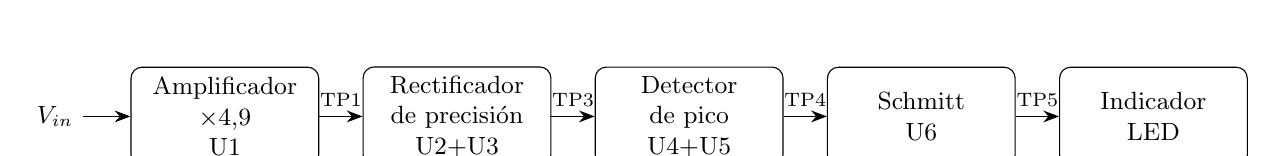
\begin{tikzpicture}[node distance=0.55cm, font=\small,
  blk/.style={draw, rounded corners, align=center, minimum height=1.25cm, text width=2.15cm},
  >={Stealth[length=2mm]}]
\node[blk] (a) {Amplificador\\$\times 4{,}9$\\U1};
\node[blk, right=of a] (b) {Rectificador de precisión\\U2+U3};
\node[blk, right=of b] (c) {Detector de pico\\U4+U5};
\node[blk, right=of c] (d) {Schmitt\\U6};
\node[blk, right=of d] (e) {Indicador\\LED};
\draw[<-] (a.west) -- ++(-0.6,0) node[left]{$V_{in}$};
\draw[->] (a) -- node[above]{\scriptsize TP1} (b);
\draw[->] (b) -- node[above]{\scriptsize TP3} (c);
\draw[->] (c) -- node[above]{\scriptsize TP4} (d);
\draw[->] (d) -- node[above]{\scriptsize TP5} (e);
\end{tikzpicture}
\caption{Diagrama de bloques del detector y puntos de prueba.}\label{fig:bloques}
\end{figure}

\subsection{Esquema eléctrico}

\begin{figure}[H]
\centering
\resizebox{\linewidth}{!}{% Esquema electrico completo del detector de latido ECG (circuitikz)
\begin{circuitikz}[european resistors, american inductors, font=\small]
\ctikzset{amplifiers/scale=0.75, diodes/scale=0.6, resistors/scale=0.7, capacitors/scale=0.7, grounds/scale=0.8}

% ================= FILA 1: amplificador + rectificador =================
% --- U1: amplificador no inversor ---
\draw (0,0) node[ocirc]{} node[left]{$V_{in}$} to[short,-*] (1,0) coordinate(nin);
\node[op amp, noinv input up, anchor=+] (U1) at (2.4,0) {U1};
\draw (nin) -- (U1.+);
\draw (nin) to[R, l_={$R_0$\ 100\,k$\Omega$}] ++(0,-2.2) node[ground]{};
\draw (U1.-) -- ++(-0.35,0) coordinate(m1) -- (m1 |- 0,-2.0) coordinate(n1);
\coordinate (vg) at ($(U1.out)+(0.6,0)$);
\draw (U1.out) to[short,-*] (vg);
\draw (n1) to[R, l={$R_{g1}$\ 10\,k$\Omega$}, *-] ++(0,-1.6) node[ground]{};
\draw (n1) to[R, l={$R_{f1}$\ 39\,k$\Omega$}] (n1 -| vg) -- (vg);
\node[above] at (vg) {$V_g$ (TP1)};

% --- U2: rectificador de media onda inversor ---
\node[op amp, anchor=-] (U2) at ($(vg)+(3.6,0)$) {U2};
\coordinate (N) at ($(U2.-)+(-0.6,0)$);
\draw (vg) to[R, l={$R_2$\ 10\,k$\Omega$}, -*] (N) -- (U2.-);
\draw (U2.+) -- ++(-0.3,0) node[ground]{};
\coordinate (o2) at ($(U2.out)+(0.45,0)$);
\draw (U2.out) to[short,-*] (o2);
\draw (N) to[short,-*] (N |- 0,1.3) coordinate(d1l);
\draw (d1l -| o2) to[D, l_={$D_1$}] (d1l);
\draw (d1l -| o2) -- (o2);
\coordinate (vhwx) at ($(o2)+(1.3,0)$);
\draw (d1l) -- (N |- 0,2.6) to[R, l={$R_3$\ 10\,k$\Omega$}, -*] (vhwx |- 0,2.6) coordinate(VHW);
\draw (VHW) to[D, l={$D_2$}] (VHW |- o2) -- (o2);
\node[above right] at (VHW) {$V_{hw}$ (TP2)};

% --- U3: sumador inversor ---
\coordinate (S) at ($(VHW)+(3.2,0)$);
\draw (VHW) to[R, l_={$R_5$\ 10\,k$\Omega$}, -*] (S);
\node[op amp, anchor=-] (U3) at ($(S |- 0,1.0)+(0.7,0)$) {U3};
\draw (S) -- (S |- U3.-) to[short,-] (U3.-);
\draw (U3.+) -- ++(-0.3,0) node[ground]{};
\coordinate (o3) at ($(U3.out)+(0.5,0)$);
\draw (U3.out) to[short,-*] (o3);
\draw (S) -- ++(0,1.2) coordinate(r6l) to[R, l={$R_6$\ 20\,k$\Omega$}] (r6l -| o3) -- (o3);
\draw (vg) to[short,*-] (vg |- 0,-4.0) to[R, l={$R_4$\ 20\,k$\Omega$}] (S |- 0,-4.0) to[short,-*] (S |- U3.-);
\node[above right] at (o3) {$V_r=|V_g|$ (TP3)};

% ================= FILA 2: detector de pico + Schmitt + salida =================
\coordinate (yrow) at (0,-8.0);
\draw (o3) -- ++(0.6,0) coordinate(o3b) -- (o3b |- 0,-5.6) -- (0.4,-5.6) coordinate(cr) -- (cr |- yrow) -- ++(1.0,0) coordinate(u4p);

% --- U4: detector ---
\node[op amp, noinv input up, anchor=+] (U4) at (u4p) {U4};
\coordinate (o4) at ($(U4.out)+(0.4,0)$);
\draw (U4.out) to[short,-*] (o4);
\draw (o4) to[D, l={$D_3$}] ++(1.6,0) to[R, l={$R_7$\ 100\,$\Omega$}] ++(2.0,0) coordinate(nc);
\draw (nc) to[C, l_={$C_1$\ 1\,$\mu$F}, *-] ++(0,-1.8) node[ground]{};
\draw (nc) to[short,-*] ++(1.4,0) coordinate(nc2);
\draw (nc2) to[R, l={$R_9$\ 100\,k$\Omega$}] ++(0,-1.8) node[ground]{};

% D4 y R8
\draw (U4.-) -- ++(-0.35,0) coordinate(a4) -- ++(0,-1.0) coordinate(d4l);
\draw (d4l) to[D, l_={$D_4$}, *-] (d4l -| o4) -- (o4);

% --- U5: buffer ---
\node[op amp, noinv input up, anchor=+] (U5) at ($(nc2)+(1.4,0)$) {U5};
\draw (nc2) -- (U5.+);
\coordinate (o5) at ($(U5.out)+(0.45,0)$);
\draw (U5.out) to[short,-*] (o5);
\draw (U5.-) -- ++(-0.3,0) -- ++(0,-0.9) -| (o5);
\coordinate (o6) at ($(o5)+(0.9,0)$);
\draw (o5) to[short,-*] (o6);
\node[above] at (o6) {$V_{env}$ (TP4)};
\draw (d4l) -- ++(0,-1.6) coordinate(r8l) to[R, l_={$R_8$\ 10\,k$\Omega$}] (r8l -| o6) -- (o6);

% --- U6: Schmitt no inversor ---
\node[op amp, noinv input up, anchor=+] (U6) at ($(o6)+(3.0,0)$) {U6};
\coordinate (P) at ($(U6.+)+(-0.45,0)$);
\draw (o6) to[R, l_={$R_{10}$\ 10\,k$\Omega$}, -*] (P) -- (U6.+);
\coordinate (o7) at ($(U6.out)+(0.5,0)$);
\draw (U6.out) to[short,-*] (o7);
\draw (P) -- ++(0,1.3) coordinate(r11l) to[R, l={$R_{11}$\ 430\,k$\Omega$}] (r11l -| o7) -- (o7);
\draw (U6.-) -- ++(-0.45,0) coordinate(q0) -- ++(0,-1.1) coordinate(Q);
\draw (Q) to[R, l={$R_{13}$\ 1\,k$\Omega$}, *-] ++(0,-1.6) node[ground]{};
\draw (Q) to[R, l_={$R_{12}$\ 15\,k$\Omega$}] ++(-1.8,0) node[left]{$+12$\,V};
\node[right] at ($(Q)+(0.05,0.25)$) {\footnotesize $V_{ref}=0{,}75$\,V};

% --- Salida ---
\draw (o7) to[D, l={$D_5$}] ++(1.5,0) coordinate(l1) to[R, l={$R_{14}$\ 1\,k$\Omega$}] ++(0,-1.8) to[led, l={LED}] ++(0,-1.5) node[ground]{};
\node[above] at (o7) {TP5};
\end{circuitikz}
}
\caption{Esquema eléctrico completo. Alimentación de $\pm\SI{12}{V}$ y desacoples de \SI{100}{nF} no dibujados.}\label{fig:esquema}
\end{figure}

La señal recorre la primera fila de izquierda a derecha y pasa a la segunda en TP3. Las conexiones de cada op-amp son:
\begin{enumerate}
  \item \textbf{U1 (amplificador):} $(+)\leftarrow$ entrada, con R0 a tierra; $(-)\leftarrow$ Rg1 a tierra y Rf1 desde la salida. Salida $=\Vg$ (TP1).
  \item \textbf{U2 (media onda):} $(+)$ a tierra; $(-)\leftarrow\Vg$ por R2. D1: ánodo en la salida de U2, cátodo en $(-)$. D2: cátodo en la salida de U2, ánodo en el nodo $V_{hw}$. R3 de $(-)$ a $V_{hw}$ (TP2).
  \item \textbf{U3 (sumador):} $(+)$ a tierra; $(-)\leftarrow\Vg$ por R4 y $\leftarrow V_{hw}$ por R5; R6 de $(-)$ a la salida. Salida $=\Vr=|\Vg|$ (TP3).
  \item \textbf{U4 (detector):} $(+)\leftarrow\Vr$. Salida $\rightarrow$ D3 $\rightarrow$ R7 $\rightarrow$ nodo de C1 (C1 y R9 en paralelo a tierra). $(-)\leftarrow\Venv$ por R8. D4: ánodo en $(-)$, cátodo en la salida de U4.
  \item \textbf{U5 (buffer):} seguidor; $(+)\leftarrow$ nodo de C1, $(-)$ unido a la salida. Salida $=\Venv$ (TP4).
  \item \textbf{U6 (Schmitt):} $(+)\leftarrow\Venv$ por R10 y $\leftarrow$ salida de U6 por R11. $(-)\leftarrow\Vref$ (divisor R12 desde $+\SI{12}{V}$, R13 a tierra). Salida $=$ TP5.
  \item \textbf{Indicador:} TP5 $\rightarrow$ D5 $\rightarrow$ R14 $\rightarrow$ LED $\rightarrow$ tierra.
\end{enumerate}

% ---------------- Etapa 1 ----------------
\subsection{Etapa 1: amplificador no inversor (U1)}

Esta etapa es la primera que se diseña: lleva la señal de entrada a un nivel cómodo para el resto del circuito, alejándola del ruido y de los offsets sin llegar a saturar.

\paragraph{Derivación.} La entrada no inversora está conectada a la señal, así que $V_+=V_{in}$. La inversora toma una fracción de la salida por el divisor Rf1--Rg1:
\begin{equation}
V_- = \Vg\,\frac{R_{g1}}{R_{g1}+R_{f1}}
\end{equation}
Igualando $V_-=V_+=V_{in}$ y despejando:
\begin{equation}
\Vg = V_{in}\left(1+\frac{R_{f1}}{R_{g1}}\right) = V_{in}\left(1+\frac{\SI{39}{k\ohm}}{\SI{10}{k\ohm}}\right) = 4{,}9\,V_{in}
\label{eq:ganancia}
\end{equation}

\paragraph{Elección de la ganancia.} Al iniciar el diseño solo se conocen la entrada (picos de 0,5 a \SI{2}{V}) y la saturación del op-amp ($\Vsat\approx\SI{10,5}{V}$); los umbrales del comparador todavía no existen. La entrada varía en una relación 4:1, así que no es posible dejar la señal grande y la pequeña en un nivel ideal a la vez. El criterio es \textbf{amplificar lo máximo posible sin que la señal más grande sature}, para que la más pequeña quede lo más lejos posible del ruido y de los offsets.

\begin{enumerate}
  \item \textbf{Límite por saturación.} La entrada máxima es el pulso de \SI{2}{V_{pp}} con nivel bajo en \SI{0}{V}, cuyo pico es \SI{2}{V}:
  \begin{equation}
  G\cdot\SI{2}{V}\le\Vsat\;\Rightarrow\;G_{max}=\frac{10{,}5}{2}=5{,}25
  \end{equation}
  Por encima de este valor el pulso sale recortado y el detector de pico deja de ver la amplitud real.
  \item \textbf{Valor comercial.} Con $R_{g1}=\SI{10}{k\ohm}$, $R_{f1}=(G-1)R_{g1}\le\SI{42,5}{k\ohm}$. En la serie E12:
  \begin{itemize}
    \item $R_{f1}=\SI{39}{k\ohm}\Rightarrow G=4{,}9$, un \SI{7}{\percent} por debajo de la saturación.
    \item $R_{f1}=\SI{47}{k\ohm}\Rightarrow G=5{,}7$, que satura.
  \end{itemize}
  Se elige $G=4{,}9$, la mayor ganancia comercial que no satura.
  \item \textbf{Rango resultante.} La señal amplificada queda con picos de
  \begin{equation}
  V_{p,min}=4{,}9\cdot0{,}5=\SI{2,45}{V},\qquad V_{p,max}=4{,}9\cdot2=\SI{9,8}{V}
  \end{equation}
  Estos valores son los datos de partida de las etapas siguientes.
  \item \textbf{Requisito que se traslada al comparador.} Para detectar la señal más pequeña con un margen de 2 veces frente a ruido y tolerancias, el umbral de disparo del Schmitt deberá cumplir
  \begin{equation}
  \VTH\le\frac{V_{p,min}}{2}=\frac{2{,}45}{2}=\SI{1,22}{V}
  \label{eq:vthmax}
  \end{equation}
  Esta condición se usa en la etapa 4.
\end{enumerate}

La figura~\ref{fig:calcgan} muestra el planteamiento a mano de este criterio: el límite por saturación ($G\le5{,}25$), la elección de $G=4{,}9$ con margen y la comprobación de los picos máximo (\SI{9,8}{V}) y mínimo (\SI{2,45}{V}) frente a $\Vsat$.

\begin{figure}[H]
\centering
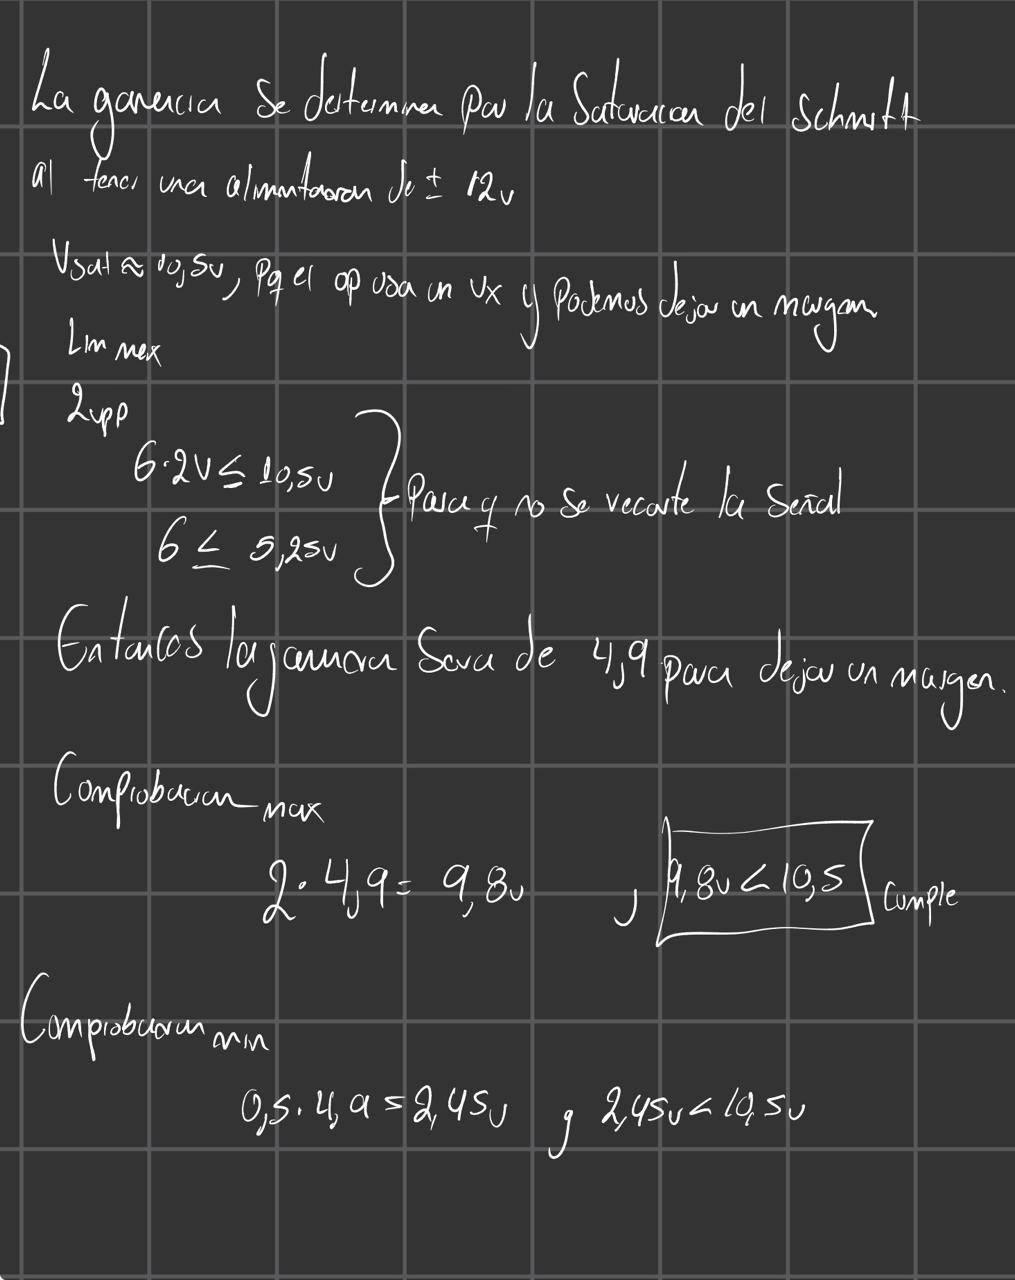
\includegraphics[width=0.62\linewidth]{calc_ganancia.png}
\caption{Planteamiento a mano: elección de la ganancia del amplificador no inversor a partir de la saturación.}\label{fig:calcgan}
\end{figure}

\paragraph{Verificación.} Con el Schmitt ya diseñado ($\VTH=\SI{1,01}{V}$, etapa 4) se comprueba que la ganancia queda dentro de la ventana que imponen ambas etapas:
\begin{equation}
\underbrace{\frac{2\cdot1{,}01}{0{,}5}}_{4{,}04}\;\le\;G=4{,}9\;\le\;\underbrace{\frac{10{,}5}{2}}_{5{,}25}
\end{equation}

\paragraph{No idealidades.} Con ganancia en lazo abierto finita,
\begin{equation}
G_{real}=\frac{G}{1+G/A_{ol}}=\frac{4{,}9}{1+4{,}9/\num{200000}}\approx 4{,}8999
\end{equation}
con un error de \SI{0,0025}{\percent}. El ancho de banda es $f_{-3dB}=GBW/G$: \SI{612}{kHz} con TL074 y \SI{204}{kHz} con LM324. El flanco de 0 a \SI{9,8}{V} tarda \SI{0,75}{\micro s} con TL074 y \SI{20}{\micro s} con LM324, despreciable frente a \SI{75}{ms}. El generador (\SI{50}{\ohm}) ve R0 $=\SI{100}{k\ohm}$: la atenuación es 0,9995.

\paragraph{Memoria de cálculo.} La figura~\ref{fig:calcamp} reproduce el cálculo hecho a mano: con $R_{g1}=\SI{10}{k\ohm}$ y $A_v=4{,}9$ se despeja $R_{f1}=(A_v-1)R_{g1}=\SI{39}{k\ohm}$.

\begin{figure}[H]
\centering
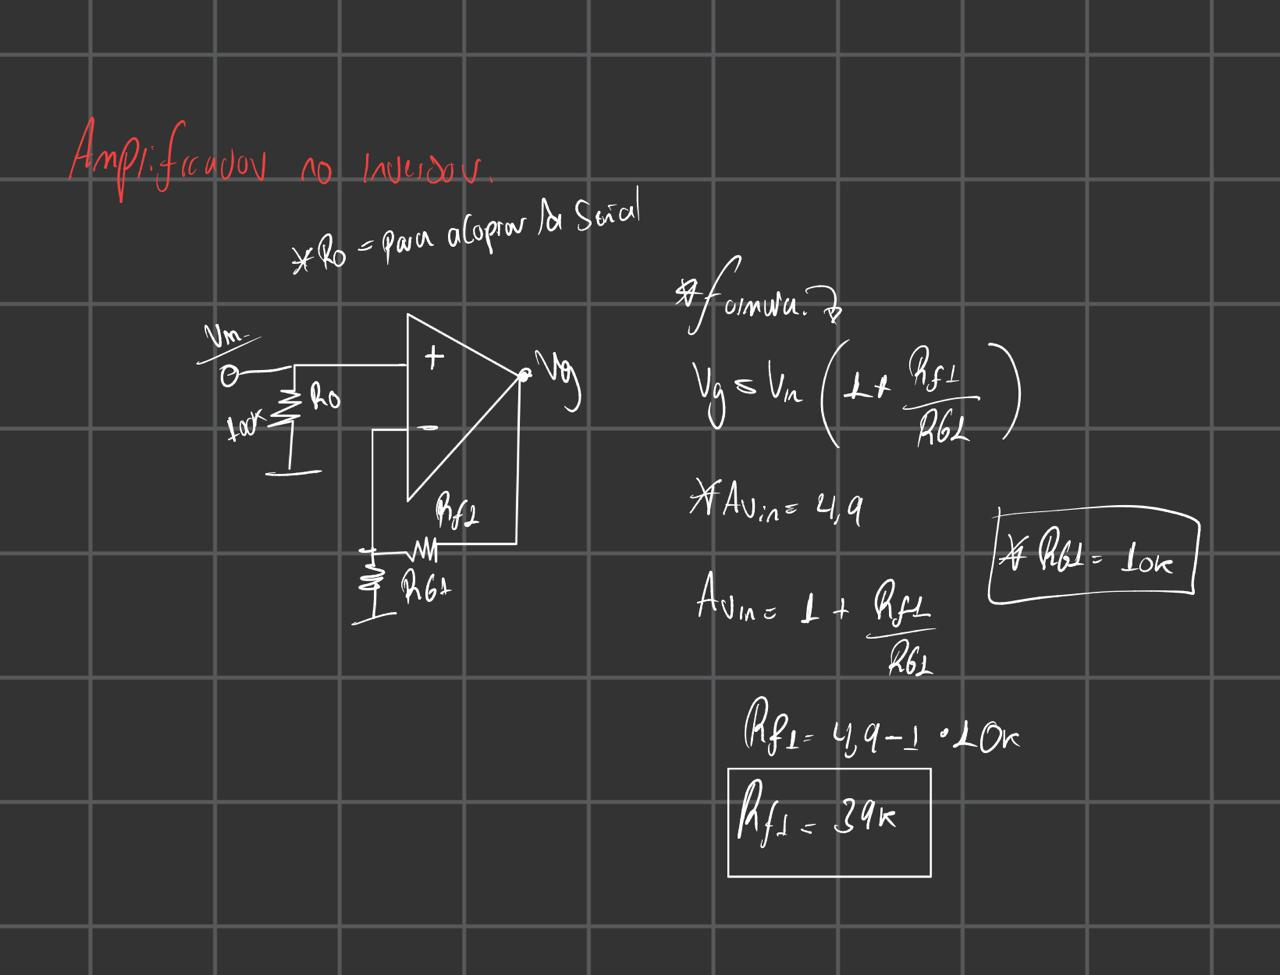
\includegraphics[width=\linewidth]{calc_amplificador.png}
\caption{Memoria de cálculo a mano: amplificador no inversor (U1).}\label{fig:calcamp}
\end{figure}

% ---------------- Etapa 2 ----------------
\subsection{Etapa 2: rectificador de precisión de onda completa (U2 + U3)}

La etapa entrega $\Vr=|\Vg|$ con ganancia 1 en ambas polaridades.

\paragraph{Semiciclo positivo ($\Vg>0$).} La entrada $(+)$ de U2 está a tierra, así que su entrada $(-)$ es tierra virtual. Por R2 entra $i=\Vg/R_2$; como no puede entrar al op-amp, sigue por R3 hacia el nodo $V_{hw}$. La salida de U2 baja, D2 conduce y D1 queda en inversa. Por la ley de corrientes en la entrada inversora:
\begin{equation}
\frac{\Vg-0}{R_2}=\frac{0-V_{hw}}{R_3}\;\Rightarrow\; V_{hw}=-\frac{R_3}{R_2}\Vg=-\Vg
\end{equation}
La salida de U2 queda una caída de diodo por debajo: $V_{hw}-\SI{0,6}{V}$. Esa caída no aparece en $V_{hw}$ porque la señal se toma después de D2, dentro del lazo.

\paragraph{Semiciclo negativo ($\Vg<0$).} La corriente por R2 sale del nodo; la salida de U2 sube hasta que D1 conduce y queda en $\approx+\SI{0,6}{V}$, casi independiente de $\Vg$. D2 queda en inversa, por R3 y R5 no circula corriente y $V_{hw}=0$.

\paragraph{Sumador (U3).} Con tierra virtual en su entrada $(-)$, la corriente por R6 es la suma de las que llegan por R4 y R5:
\begin{equation}
\frac{\Vg}{R_4}+\frac{V_{hw}}{R_5}=-\frac{\Vr}{R_6}\;\Rightarrow\;\Vr=-\left(\frac{R_6}{R_4}\Vg+\frac{R_6}{R_5}V_{hw}\right)=-\left(\Vg+2V_{hw}\right)
\label{eq:sumador}
\end{equation}
Sustituyendo cada semiciclo:
\begin{equation}
\Vg>0:\;\Vr=-(\Vg-2\Vg)=+\Vg \qquad \Vg<0:\;\Vr=-(\Vg+0)=-\Vg
\end{equation}
En ambos casos $\Vr=|\Vg|$. El camino por R4 lleva la señal completa (antes del rectificador) con peso 1; el camino por R5 lleva la media onda con peso 2, que en el semiciclo positivo anula el término equivocado y lo vuelve a sumar con el signo correcto.

\begin{table}[H]
\centering
\caption{Tensiones y estado de los diodos con $\Vg=\pm\SI{4}{V}$.}\label{tab:rect4}
\begin{tabular}{@{}lcc@{}}
\toprule
 & $\Vg=+\SI{4}{V}$ & $\Vg=-\SI{4}{V}$ \\
\midrule
Salida de U2 & $-\SI{4,6}{V}$ & $\approx+\SI{0,62}{V}$ \\
D1 / D2 & Corte / conduce & Conduce / corte \\
$V_{hw}$ (TP2) & $-\SI{4}{V}$ & \SI{0}{V} \\
Corriente por D2 & \SI{0,8}{mA} (R3 + R5) & 0 \\
$\Vr$ (TP3) & $+\SI{4}{V}$ & $+\SI{4}{V}$ \\
\bottomrule
\end{tabular}
\end{table}

\begin{figure}[H]
\centering
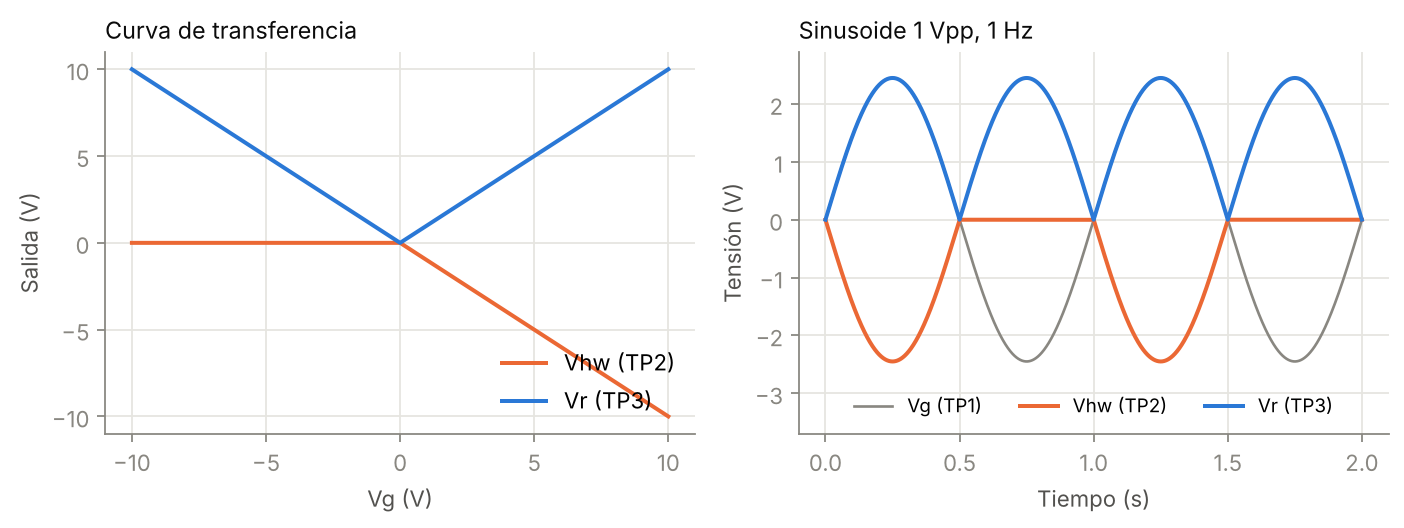
\includegraphics[width=\linewidth]{f1_rectificador.png}
\caption{Rectificador: curva de transferencia (izquierda) y formas de onda con una sinusoide (derecha).}\label{fig:rect}
\end{figure}

\paragraph{Zona muerta y transición.} Para que el diodo conduzca basta una diferencia entre entradas de
\begin{equation}
V_{zona\,muerta}=\frac{V_D}{A_{ol}}=\frac{\SI{0,6}{V}}{\num{200000}}=\SI{3}{\micro V}
\end{equation}
D1 evita que U2 se sature: sin él, en el semiciclo negativo el lazo quedaría abierto y la salida subiría a $+\SI{10,5}{V}$. Con D1 la salida solo salta \SI{1,2}{V} en cada cruce por cero, lo que tarda \SI{0,09}{\micro s} con TL074 y \SI{2,4}{\micro s} con LM324.

\paragraph{Sensibilidad a tolerancias.} Sin suponer resistencias iguales:
\begin{equation}
G_+=\frac{R_6}{R_5}\cdot\frac{R_3}{R_2}-\frac{R_6}{R_4},\qquad G_-=\frac{R_6}{R_4}
\end{equation}
$G_+$ es la resta $2-1$, que arrastra completo el error de cada término. Evaluando las 32 combinaciones de $\pm$tolerancia y una simulación Monte Carlo de \num{20000} circuitos:

\begin{table}[H]
\centering
\caption{Diferencia entre las ganancias de cada semiciclo según la tolerancia.}\label{tab:tol}
\begin{tabular}{@{}lcc@{}}
\toprule
Resistencias & Peor caso $|G_+-G_-|/G_-$ & Percentil 95 \\
\midrule
\SI{1}{\percent} & \SI{8,2}{\percent} & \SI{2,6}{\percent} \\
\SI{5}{\percent} & \SI{44}{\percent} & \SI{13}{\percent} \\
\bottomrule
\end{tabular}
\end{table}

\paragraph{Memoria de cálculo.} Las figuras~\ref{fig:calcrect} y~\ref{fig:calcsum} muestran el análisis a mano de la media onda en cada semiciclo (con el ejemplo $\Vg=\pm\SI{4}{V}$) y del sumador, de donde salen las condiciones $R_3=R_2$, $R_6=R_4$ y $R_6=2R_5$.

\begin{figure}[H]
\centering
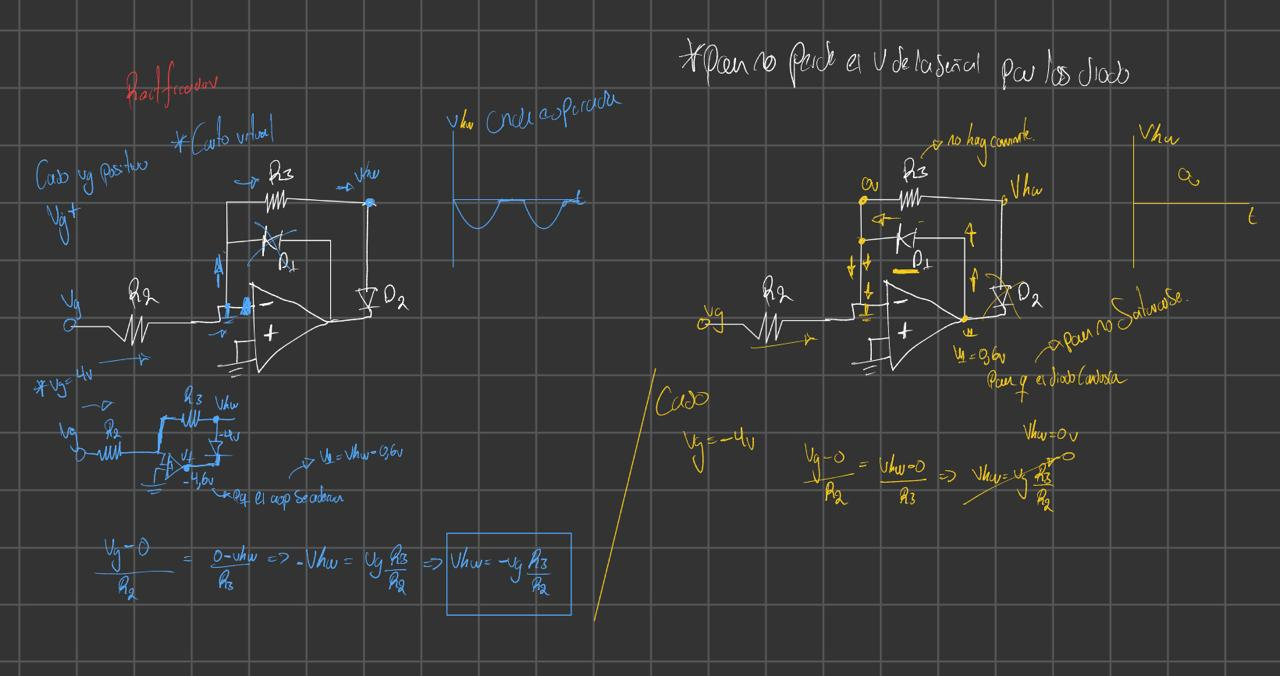
\includegraphics[width=\linewidth]{calc_rectificador.png}
\caption{Memoria de cálculo a mano: rectificador de media onda (U2) con $\Vg$ positivo y negativo.}\label{fig:calcrect}
\end{figure}

\begin{figure}[H]
\centering
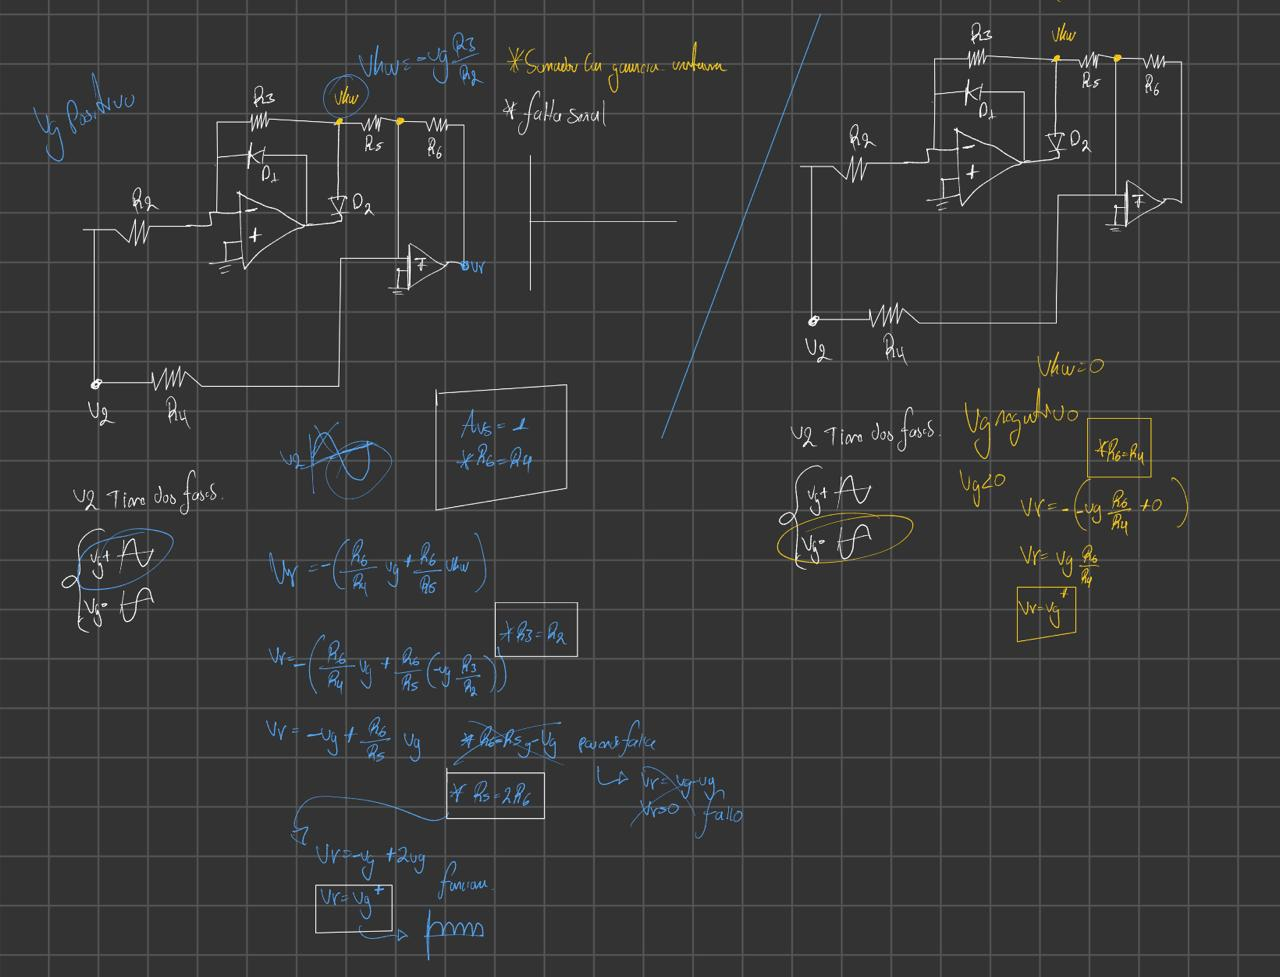
\includegraphics[width=\linewidth]{calc_sumador.png}
\caption{Memoria de cálculo a mano: sumador inversor (U3) y condiciones sobre R4, R5 y R6.}\label{fig:calcsum}
\end{figure}

% ---------------- Etapa 3 ----------------
\subsection{Etapa 3: detector de pico (U4 + U5, C1, R9)}

El detector sigue la subida de $\Vr$ en menos de \SI{1}{ms}, la mantiene mientras dura el pulso y luego descarga C1 con $\tau=\SI{100}{ms}$.

\begin{table}[H]
\centering
\caption{Datos de partida del detector de pico.}\label{tab:datos3}
\begin{tabularx}{\linewidth}{@{}llX@{}}
\toprule
Dato & Valor & Origen \\
\midrule
Pico de $\Vr$ & 2,45 a \SI{9,8}{V} & Entrada de 0,5 a \SI{2}{V_{pp}} por la ganancia de 4,9 \\
Ancho del pulso ($w$) & \SI{75}{ms} & Pulso de prueba, similar a un QRS \\
Separación entre lóbulos del QRS & $\approx\SI{20}{ms}$ & Tiempo típico entre las ondas R y S \\
Caída máxima entre lóbulos & \SI{20}{\percent} & Criterio de diseño \\
Frecuencia cardiaca máxima & 150 lpm ($T=\SI{400}{ms}$) & Rango de diseño \\
Umbral de liberación & $\VTL=\SI{0,52}{V}$ & Etapa 4 \\
Corriente máxima del op-amp & $\approx\SI{20}{mA}$ & Hoja de datos \\
Corriente de polarización & $\approx\SI{80}{nA}$ & Hoja de datos del 741 (peor caso) \\
\bottomrule
\end{tabularx}
\end{table}

\subsubsection{Funcionamiento}

\paragraph{Carga ($\Vr>\Venv$).} U4 compara $\Vr$ (entrada $+$) con $\Venv$, que le llega por R8 desde el buffer U5 (entrada $-$). Si $\Vr$ es mayor, la salida de U4 sube, D3 conduce y C1 se carga por R7 hasta $\Venv=\Vr$. Como R8 toma la tensión después de D3, la caída del diodo queda dentro del lazo: la salida de U4 se coloca $\approx\SI{0,5}{V}$ por encima de $\Venv$ y $\Venv$ sale igual a $\Vr$. La carga la limita la corriente máxima del op-amp:
\begin{equation}
\frac{d\Venv}{dt}=\frac{I_{max}}{C_1}=\frac{\SI{20}{mA}}{\SI{1}{\micro F}}=\SI{20}{V/ms}
\end{equation}
Llegar a \SI{9,8}{V} toma $\approx\SI{0,5}{ms}$.

\paragraph{Descarga ($\Vr<\Venv$).} Al terminar el pulso $\Vr$ cae a cero de inmediato, pero C1 no puede cambiar su tensión de golpe. D3 queda en inversa y la entrada del buffer no consume corriente, así que C1 solo se descarga por R9:
\begin{equation}
C_1\frac{d\Venv}{dt}=-\frac{\Venv}{R_9}\;\Rightarrow\;\Venv(t)=V_p\,e^{-t/\tau},\qquad \tau=R_9C_1
\label{eq:descarga}
\end{equation}
D4 cierra el lazo de U4: su entrada $(-)$ queda en $\Vr=0$ y su salida en $\approx-\SI{0,6}{V}$, sin saturarse. La diferencia entre $\Venv$ y esa entrada cae en R8 (\SI{0,4}{mA} con $\Venv=\SI{4}{V}$), y esa corriente la entrega el buffer, no C1.

\paragraph{Función del buffer.} U5 es un seguidor ($V_{out}=V_{in}$, impedancia de entrada del orden de $10^{11}\,\Omega$). Sin él, C1 se descargaría también por R8 y $\tau$ caería a $(R_9\parallel R_8)C_1\approx\SI{9}{ms}$; la envolvente bajaría entre los lóbulos del QRS y un latido daría varios pulsos.

\paragraph{Tiempo hasta liberar el comparador.} De $V_p\,e^{-t/\tau}=\VTL$:
\begin{equation}
t_{desc}=\tau\,\ln\frac{V_p}{\VTL}
\label{eq:tdesc}
\end{equation}

\begin{table}[H]
\centering
\caption{Tiempo de descarga y ancho del pulso de salida.}\label{tab:tdesc}
\begin{tabular}{@{}cccc@{}}
\toprule
Entrada & $V_p$ & $t_{desc}$ & Ancho de salida ($w+t_{desc}$) \\
\midrule
\SI{0,5}{V_{pp}} & \SI{2,45}{V} & \SI{154}{ms} & \SI{229}{ms} \\
\SI{1}{V_{pp}} & \SI{4,90}{V} & \SI{224}{ms} & \SI{299}{ms} \\
\SI{2}{V_{pp}} & \SI{9,80}{V} & \SI{293}{ms} & \SI{368}{ms} \\
\bottomrule
\end{tabular}
\end{table}

\begin{figure}[H]
\centering
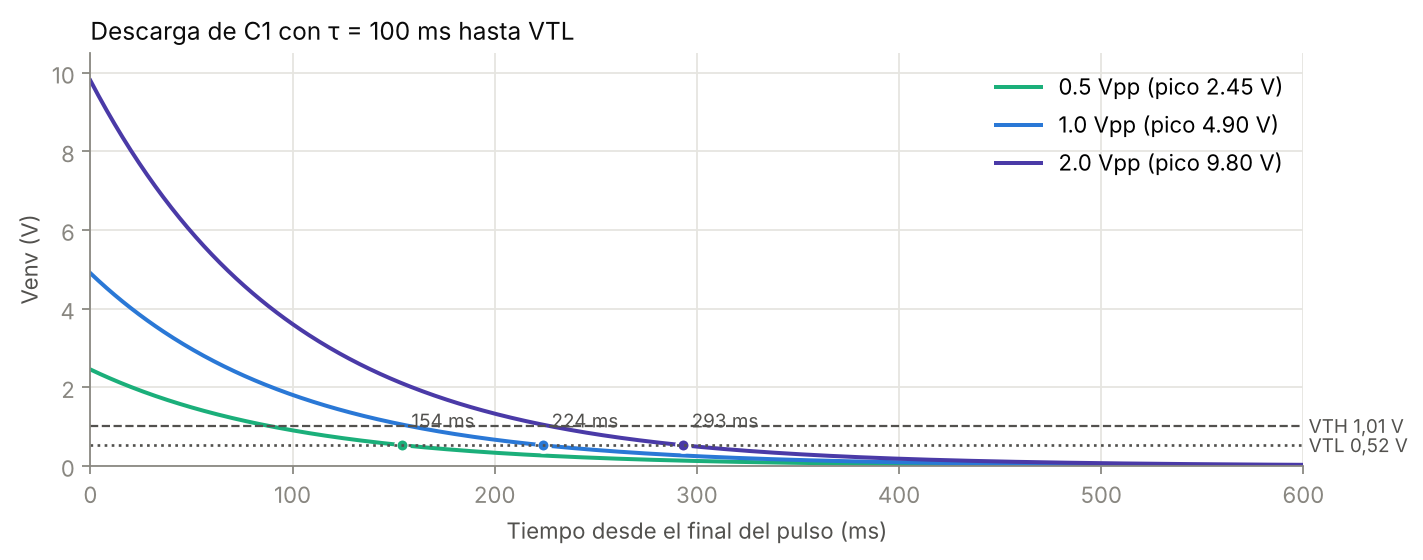
\includegraphics[width=\linewidth]{f3_descarga.png}
\caption{Descarga de C1 hasta $\VTL$ para las tres amplitudes.}\label{fig:descarga}
\end{figure}

\subsubsection{Diseño de los componentes}

\paragraph{Límite inferior de $\tau$.} El QRS no es un pulso único: sus lóbulos (Q, R y S) están separados unos \SI{20}{ms} y el complejo completo dura de 80 a \SI{120}{ms} en un adulto~\cite{guyton}. Entre lóbulos la envolvente no debe perder más del \SI{20}{\percent} (criterio de diseño), para que el comparador no se libere en medio del complejo y cuente un latido dos veces:
\begin{equation}
e^{-\SI{20}{ms}/\tau}>0{,}8\;\Rightarrow\;\tau>\frac{\SI{20}{ms}}{\ln(1/0{,}8)}\approx\SI{90}{ms}
\end{equation}

\paragraph{Condición de descarga.} La condición para el límite superior se deduce siguiendo un latido completo:
\begin{enumerate}
  \item \textbf{Carga.} Llega el pulso y C1 se carga al pico $V_p$ en $\approx\SI{0,1}{ms}$ ($R_7C_1$). $\Venv$ supera $\VTH$ y la salida del Schmitt sube.
  \item \textbf{Retención.} Mientras dura el pulso ($w$), U4 mantiene C1 en $V_p$.
  \item \textbf{Descarga.} Al terminar el pulso, D3 se bloquea y C1 se descarga solo por R9, con la respuesta natural de un circuito RC~\cite{sedra,boylestad}: $\Venv(t)=V_p\,e^{-t/\tau}$.
  \item \textbf{Liberación.} El Schmitt vuelve a bajo cuando $\Venv=\VTL$~\cite{sedra}, lo que ocurre después del tiempo de descarga $t_{desc}=\tau\ln(V_p/\VTL)$ de la ecuación~\eqref{eq:tdesc}.
\end{enumerate}
Desde que empieza un latido hasta que el comparador queda listo para el siguiente pasan $w+t_{desc}$. Si el siguiente latido llega antes, $\Venv$ sigue por encima de $\VTL$, la salida no baja y los dos latidos se cuentan como uno. La condición para detectar cada latido por separado es entonces
\begin{equation}
w+\tau\ln\frac{V_p}{\VTL}<T=\frac{60}{FC}
\label{eq:condesc}
\end{equation}
Este tiempo cumple la misma función que el \emph{periodo refractario} de los detectores de QRS por software, que ignoran cualquier evento durante unos \SI{200}{ms} después de cada latido~\cite{pantompkins}. Aquí el periodo refractario no se programa: lo fijan $\tau$, $V_p$ y $\VTL$.

\paragraph{Límite superior de $\tau$.} El peor caso es el pico más alto (\SI{9,8}{V}, que tarda más en descargarse) a la frecuencia más alta del enunciado (150 lpm, $T=\SI{400}{ms}$). Con $\VTL=\SI{0,52}{V}$ (etapa 4) en la ecuación~\eqref{eq:condesc}:
\begin{equation}
\SI{75}{ms}+\tau\ln\frac{9{,}8}{0{,}52}<\SI{400}{ms}\;\Rightarrow\;\tau<\frac{\SI{325}{ms}}{2{,}94}\approx\SI{110}{ms}
\end{equation}

Se elige el punto medio de la ventana \SIrange{90}{110}{ms}, $\tau=\SI{100}{ms}$.

\paragraph{Frecuencia cardiaca máxima.} Despejando $FC$ de la ecuación~\eqref{eq:condesc} se obtiene la frecuencia máxima que el circuito puede contar para cualquier amplitud:
\begin{equation}
FC_{max}=\frac{60}{w+\tau\ln(V_p/\VTL)}\ \text{lpm}
\label{eq:fcmax}
\end{equation}

\begin{table}[H]
\centering
\caption{Frecuencia cardiaca máxima con $\tau=\SI{100}{ms}$, $w=\SI{75}{ms}$ y $\VTL=\SI{0,523}{V}$.}\label{tab:fcmax}
\begin{tabular}{@{}cccccc@{}}
\toprule
Entrada & $V_p$ & $V_p/\VTL$ & $t_{desc}=\tau\ln(V_p/\VTL)$ & $w+t_{desc}$ & $FC_{max}$ \\
\midrule
\SI{0,5}{V_{pp}} & \SI{2,45}{V} & 4,68 & \SI{154}{ms} & \SI{229}{ms} & 262 lpm \\
\SI{1}{V_{pp}} & \SI{4,9}{V} & 9,37 & \SI{224}{ms} & \SI{299}{ms} & 201 lpm \\
\SI{2}{V_{pp}} & \SI{9,8}{V} & 18,7 & \SI{293}{ms} & \SI{368}{ms} & 163 lpm \\
\bottomrule
\end{tabular}
\end{table}

Ejemplo con \SI{2}{V_{pp}}: $t_{desc}=0{,}1\ln(18{,}7)=\SI{0,293}{s}$, $w+t_{desc}=\SI{0,368}{s}$ y $FC_{max}=60/0{,}368=163$ lpm. Cuanto mayor es el pico, más tarda C1 en bajar hasta $\VTL$, por eso la frecuencia máxima disminuye con la amplitud. En todos los casos queda por encima de los 150 lpm del enunciado.

\begin{figure}[H]
\centering
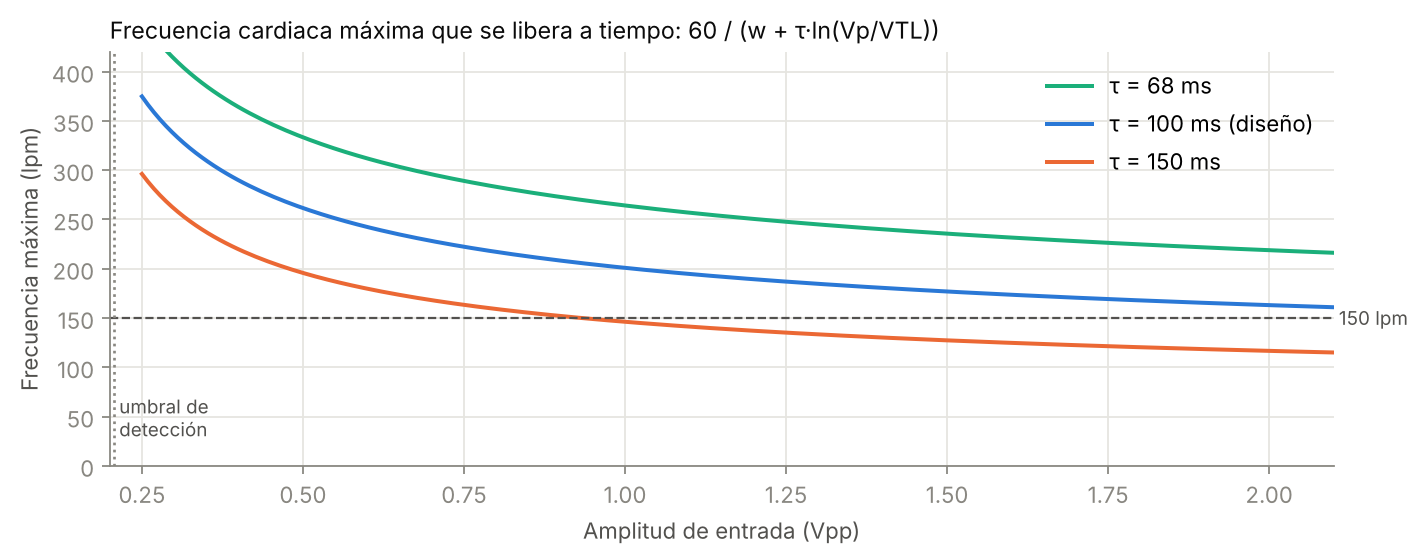
\includegraphics[width=\linewidth]{f4_fmax.png}
\caption{Frecuencia cardiaca máxima frente a la amplitud de entrada para tres valores de $\tau$.}\label{fig:fmax}
\end{figure}

\paragraph{C1 y R9.} El producto de \SI{100}{ms} admite varias combinaciones:

\begin{table}[H]
\centering
\caption{Opciones para formar $\tau=\SI{100}{ms}$.}\label{tab:c1r9}
\begin{tabularx}{\linewidth}{@{}llX@{}}
\toprule
C1 & R9 & Resultado \\
\midrule
\SI{10}{\micro F} & \SI{10}{k\ohm} & Descartado: un electrolítico tiene fugas de \si{\micro A} y $\pm\SI{20}{\percent}$ de tolerancia \\
\SI{1}{\micro F} & \SI{100}{k\ohm} & Elegido: poliéster estable; error por polarización $\SI{80}{nA}\times\SI{100}{k\ohm}=\SI{8}{mV}$ \\
\SI{100}{nF} & \SI{1}{M\ohm} & Descartado: error por polarización de \SI{80}{mV}, el \SI{15}{\percent} de $\VTL$ \\
\bottomrule
\end{tabularx}
\end{table}

\paragraph{R7 y R8.} R7 debe dar una carga mucho más rápida que la subida del QRS ($\tau_c=R_7C_1\le\SI{1}{ms}$, es decir $R_7\le\SI{1}{k\ohm}$) y aislar al op-amp de la carga capacitiva (más de $\approx\SI{50}{\ohm}$); se eligió \SI{100}{\ohm}. Por R8 circula durante la descarga $(\Venv-\Vr)/R_8$, como máximo \SI{0,98}{mA} con \SI{10}{k\ohm}; con resistencias de M$\Omega$ la corriente de polarización crearía errores de decenas de mV. Su rango útil es de \SI{1}{k\ohm} a \SI{100}{k\ohm} y se eligió \SI{10}{k\ohm}.

\begin{table}[H]
\centering
\caption{Resumen del dimensionamiento del detector.}\label{tab:res3}
\begin{tabular}{@{}llll@{}}
\toprule
Componente & Condición que lo fija & Rango válido & Valor \\
\midrule
$\tau=R_9C_1$ & Fundir el QRS y liberarse a 150 lpm & 90--\SI{110}{ms} & \SI{100}{ms} \\
C1 & Película estable & --- & \SI{1}{\micro F} \\
R9 & $\tau/C_1$ & --- & \SI{100}{k\ohm} \\
R7 & Carga rápida y estabilidad & \SI{100}{\ohm}--\SI{1}{k\ohm} & \SI{100}{\ohm} \\
R8 & Corriente del buffer y polarización & \SI{1}{k\ohm}--\SI{100}{k\ohm} & \SI{10}{k\ohm} \\
\bottomrule
\end{tabular}
\end{table}

\subsubsection{Comportamiento con sinusoide}
Con $\Vr=A|\sin\omega t|$ la envolvente sigue a la señal mientras esta cae más despacio que la exponencial y se separa cuando $\tan\varphi<\omega\tau$. En el cruce por cero queda aproximadamente en
\begin{equation}
V_{env,min}\approx A\sin\varphi_0\,e^{-\varphi_0/(\omega\tau)},\qquad \varphi_0=\arctan(\omega\tau)
\end{equation}
Con $A=\SI{4,9}{V}$: a \SI{0,5}{Hz}, $V_{env,min}\approx\SI{0,56}{V}$ (la simulación da \SI{0,42}{V}) y se ven dos pulsos por ciclo; a \SI{1}{Hz}, $V_{env,min}\approx\SI{1,07}{V}>\VTL$ y el comparador se queda en alto. Por eso la prueba con sinusoide se hace a \SI{0,5}{Hz}.

\paragraph{Memoria de cálculo.} La figura~\ref{fig:calcdet} recoge el análisis a mano de la carga y la descarga, la ecuación de $\Venv(t)$ y el cálculo de $C_1=\SI{1}{\micro F}$ y $R_9=\SI{100}{k\ohm}$.

\begin{figure}[H]
\centering
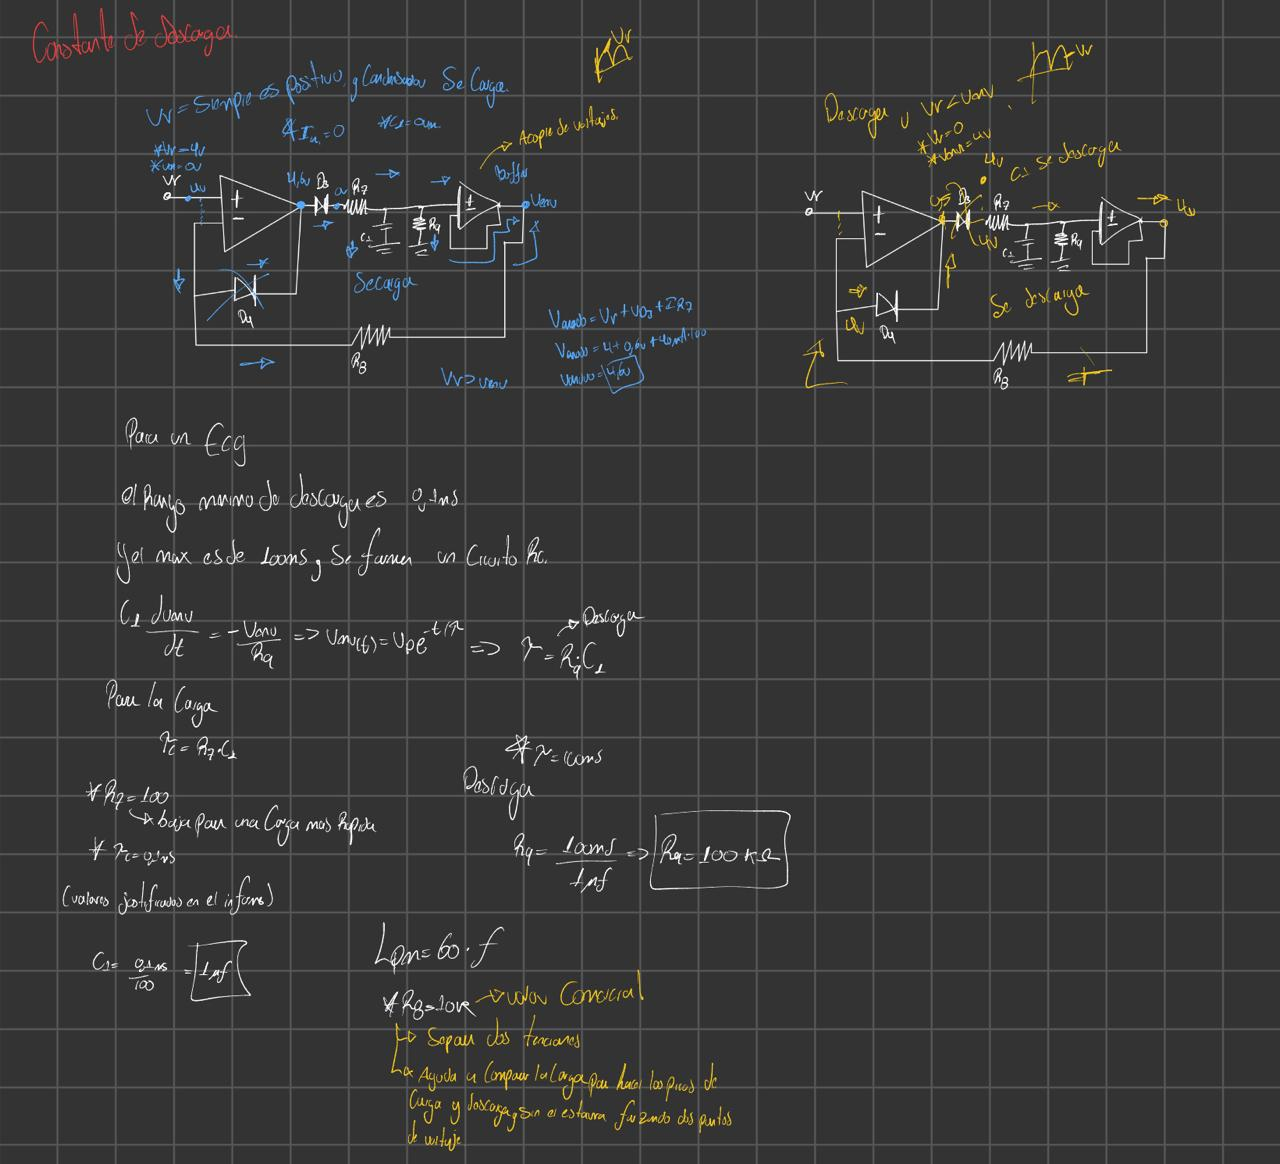
\includegraphics[width=\linewidth]{calc_detector.png}
\caption{Memoria de cálculo a mano: detector de pico (U4, U5), carga, descarga y constante de tiempo.}\label{fig:calcdet}
\end{figure}

% ---------------- Etapa 4 ----------------
\subsection{Etapa 4: comparador Schmitt no inversor (U6)}

\paragraph{Elección de los umbrales.} Esta etapa se diseña justo después de la etapa 1, porque sus umbrales dependen del pico mínimo de la señal amplificada ($V_{p,min}=\SI{2,45}{V}$) y la etapa 3 necesita conocer $\VTL$. Los umbrales se eligen con margen respecto a las señales:
\begin{itemize}
  \item $\VTH\approx\SI{1}{V}$, que cumple la condición~\eqref{eq:vthmax} ($\VTH\le\SI{1,22}{V}$): queda a la mitad o menos del pico mínimo con pulso (\SI{2,45}{V}) y por debajo del pico de la sinusoide de \SI{0,5}{V_{pp}} (\SI{1,22}{V}).
  \item $\VTL\approx\SI{0,5}{V}$, muy por encima del offset acumulado en $\Venv$ (decenas de mV) y por debajo de la onda T.
  \item $\Delta V\approx\SI{0,5}{V}$, unas diez veces el ruido esperado sobre la envolvente.
\end{itemize}

\paragraph{Ecuaciones.} U6 no tiene realimentación negativa: su salida está siempre en $\pm\Vsat$ y no hay corto virtual. Por superposición, con $k=R_{10}/R_{11}$:
\begin{equation}
V_+=\Venv\,\frac{R_{11}}{R_{10}+R_{11}}+V_o\,\frac{R_{10}}{R_{10}+R_{11}}
\end{equation}
La salida conmuta cuando $V_+=\Vref$:
\begin{equation}
\Venv=\Vref(1+k)-V_o\,k
\end{equation}
Con $V_o=-\Vsat$ (antes del latido) y $V_o=+\Vsat$ (durante el latido):
\begin{equation}
\VTH=\Vref(1+k)+\Vsat\,k,\qquad \VTL=\Vref(1+k)-\Vsat\,k
\end{equation}
\begin{equation}
\Delta V=\VTH-\VTL=2\Vsat\,k,\qquad V_c=\frac{\VTH+\VTL}{2}=\Vref(1+k)
\label{eq:hist}
\end{equation}

\paragraph{Dimensionamiento.}
\begin{enumerate}
  \item $k=\Delta V/(2\Vsat)=0{,}5/21=0{,}0238$. Con $R_{10}=\SI{10}{k\ohm}$: $R_{11}=R_{10}/k=\SI{420}{k\ohm}\rightarrow\SI{430}{k\ohm}$ (E24), $k=0{,}02326$.
  \item $\Vref=V_c/(1+k)\approx\SI{0,75}{V}$. Con el divisor desde $+\SI{12}{V}$: $R_{13}/(R_{12}+R_{13})=1/16$, es decir $R_{12}=\SI{15}{k\ohm}$ y $R_{13}=\SI{1}{k\ohm}$.
\end{enumerate}
Con los valores comerciales:
\begin{equation}
\VTH=0{,}750(1{,}02326)+10{,}5(0{,}02326)=0{,}767+0{,}244=\SI{1,012}{V}
\end{equation}
\begin{equation}
\VTL=0{,}767-0{,}244=\SI{0,523}{V},\qquad \Delta V=\SI{0,488}{V}
\end{equation}

\begin{figure}[H]
\centering
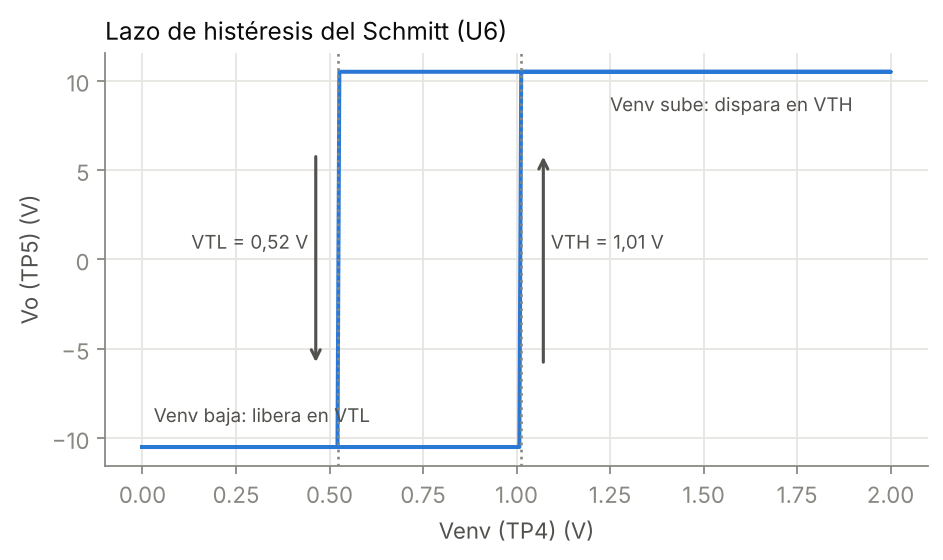
\includegraphics[width=0.7\linewidth]{f5_histeresis.png}
\caption{Lazo de histéresis del comparador: $V_o$ frente a $\Venv$.}\label{fig:hist}
\end{figure}

\paragraph{Realimentación regenerativa.} Al disparar, el término $V_o\,k$ cambia de $-\SI{0,244}{V}$ a $+\SI{0,244}{V}$ y $V_+$ salta de \SI{0,75}{V} a \SI{1,228}{V}, muy lejos de $\Vref$. Por eso el ruido no puede devolver la salida. La corriente por R11 y R10 (unos \SI{15}{\micro A}) la entrega el buffer U5, de modo que no altera la descarga de C1.

\paragraph{Sensibilidad.} Un voltio de cambio en $\Vsat$ mueve cada umbral \SI{23}{mV}; un error de $\pm\SI{5}{\percent}$ en el riel de $+\SI{12}{V}$ los mueve $\pm\SI{38}{mV}$.

\paragraph{Memoria de cálculo.} La figura~\ref{fig:calcsch} muestra el cálculo a mano de los umbrales, de $R_{11}$ a partir de la histéresis, del divisor $R_{12}$--$R_{13}$ y la verificación de $\VTH$ y $\VTL$.

\begin{figure}[H]
\centering
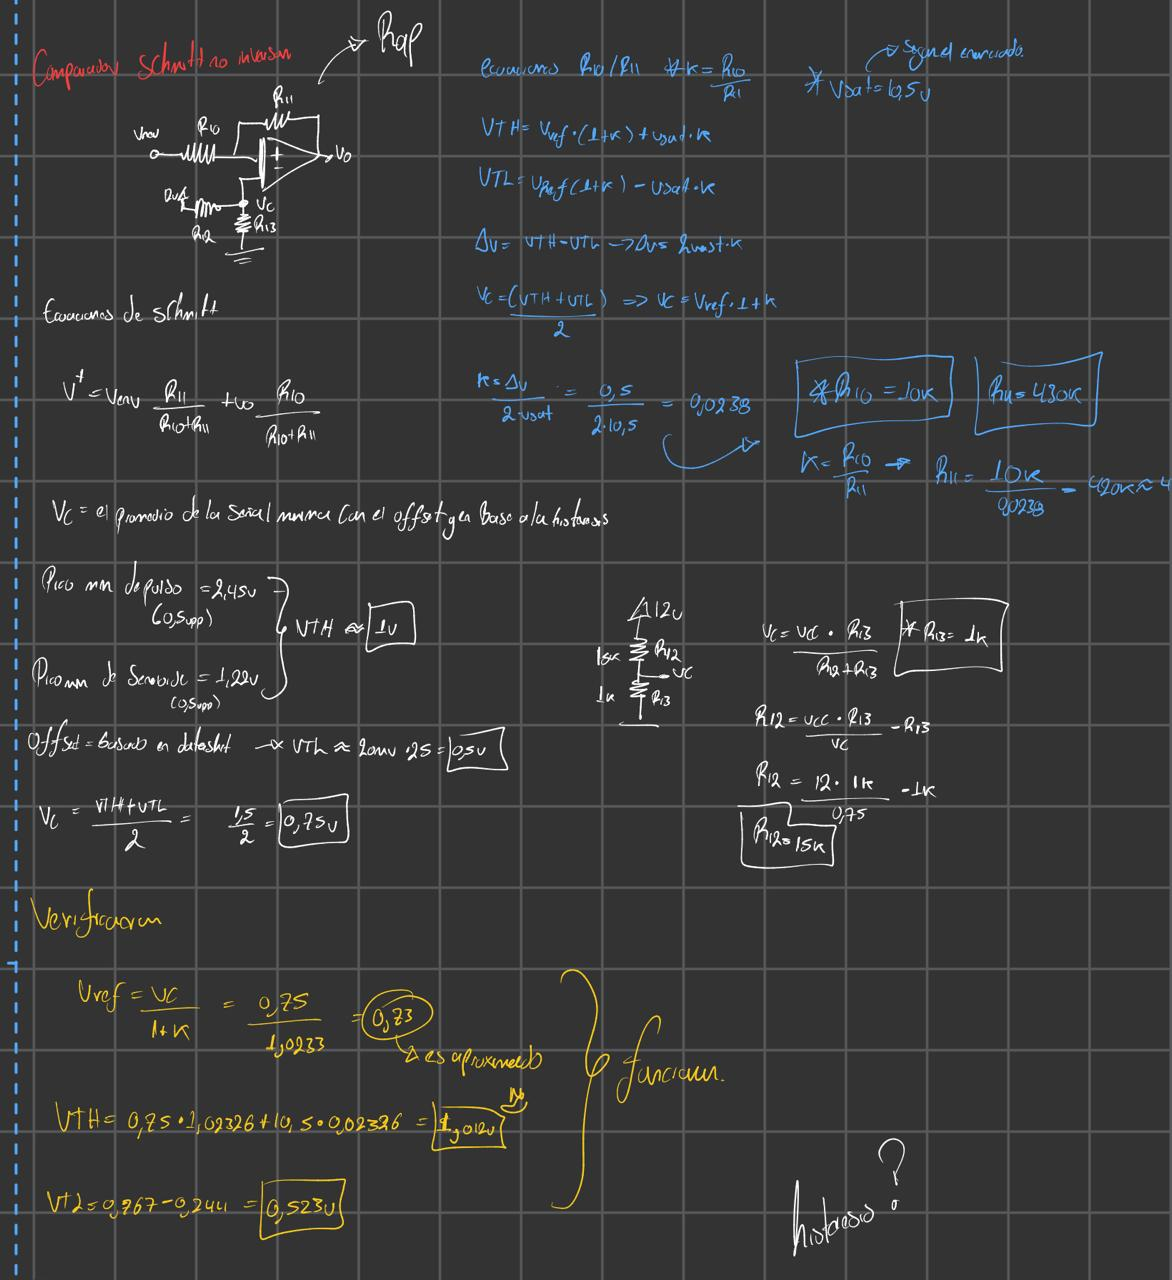
\includegraphics[width=0.88\linewidth]{calc_schmitt.png}
\caption{Memoria de cálculo a mano: comparador Schmitt no inversor (U6) y divisor de referencia.}\label{fig:calcsch}
\end{figure}

% ---------------- Etapa 5 ----------------
\subsection{Etapa 5: indicador LED}

Con $V_o=+\SI{10,5}{V}$ conducen D5 y el LED:
\begin{equation}
I_{LED}=\frac{\Vsat-V_{D5}-V_{LED}}{R_{14}}=\frac{10{,}5-0{,}7-2{,}0}{\SI{1}{k\ohm}}=\SI{7,8}{mA}
\end{equation}
La caída de D5 (\SI{0,7}{V}) es la de un diodo de silicio a corriente de mA, y la del LED rojo (\SI{2}{V}) es dato de su hoja de datos. Con $V_o=-\SI{10,5}{V}$, D5 bloquea la tensión inversa (el 1N4148 soporta \SI{100}{V}) y protege al LED, que solo tolera unos \SI{5}{V} en inversa.

La frecuencia cardiaca se obtiene contando los flancos de subida de TP5: $FC = 60/T_{RR}$, con $T_{RR}$ el tiempo entre dos flancos.

% ---------------------------- 6. SIMULACION --------------------------
\section{Simulación}

\subsection{Simulación por comportamiento (Python)}

Cada etapa se programó con las ecuaciones de la sección anterior a \num{20000} muestras por segundo (código en el anexo~\ref{anx:codigo}): ganancia de 4,9 con recorte en $\pm\SI{10,5}{V}$, rectificación ideal, carga con $\tau_c=\SI{0,1}{ms}$ y descarga exponencial con $\tau=\SI{100}{ms}$, y comparador con estado. No incluye slew rate ni caída de los diodos, que a estas frecuencias pesan menos del \SI{1}{\percent}.

\begin{figure}[H]
\centering
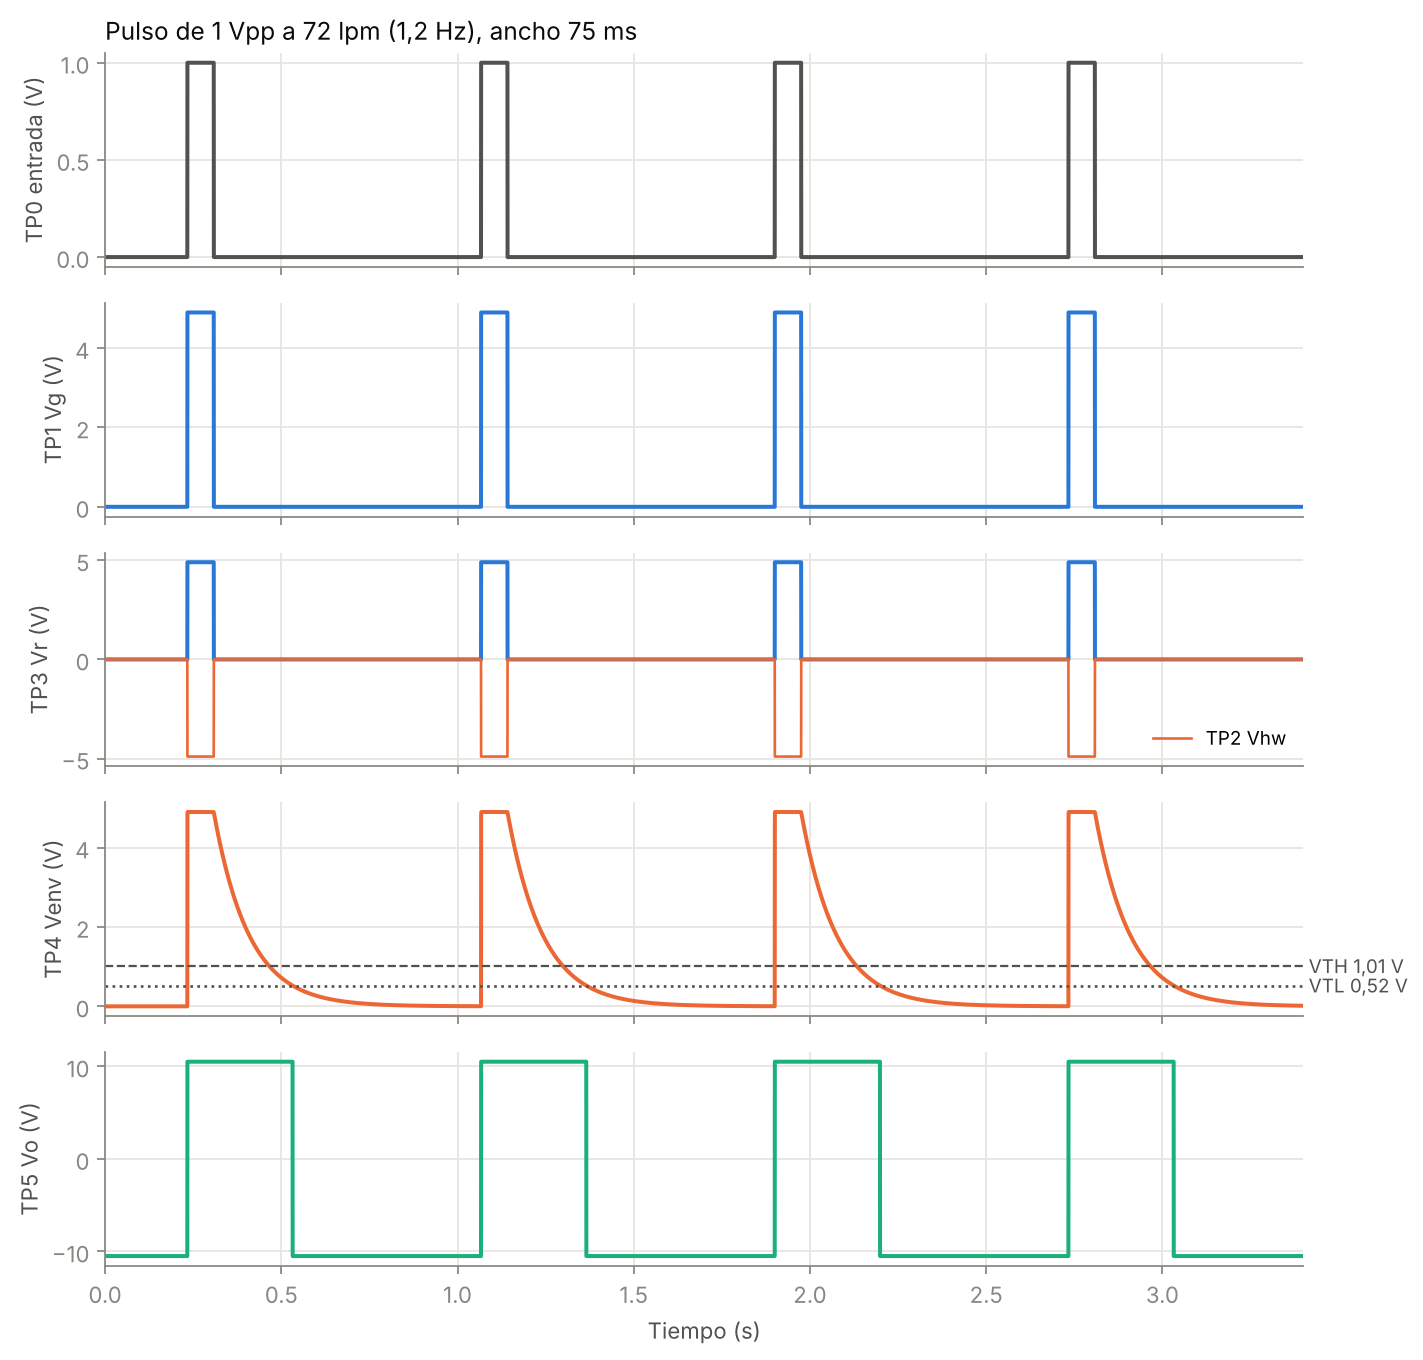
\includegraphics[width=0.95\linewidth]{f2_pulso_72lpm.png}
\caption{Formas de onda en TP0 a TP5 con un pulso de \SI{1}{V_{pp}} a 72 lpm.}\label{fig:pulso}
\end{figure}

{\small\setlength{\tabcolsep}{4pt}
\begin{longtable}{@{}ccccccc@{}}
\caption{Barrido de frecuencia y amplitud con pulso (polaridad positiva y negativa dieron resultados idénticos).}\label{tab:barrido}\\
\toprule
FC (lpm) & Entrada (V$_{pp}$) & Latidos & Detectados & Ancho (ms) & Pico $\Venv$ (V) & $\Venv$ previo (V) \\
\midrule
\endfirsthead
\toprule
FC (lpm) & Entrada (V$_{pp}$) & Latidos & Detectados & Ancho (ms) & Pico $\Venv$ (V) & $\Venv$ previo (V) \\
\midrule
\endhead
40 & 0,5 & 6 & 6 & 229 & 2,45 & 0,00 \\
40 & 1,0 & 6 & 6 & 299 & 4,90 & 0,00 \\
40 & 2,0 & 6 & 6 & 368 & 9,79 & 0,00 \\
72 & 0,5 & 12 & 12 & 229 & 2,45 & 0,00 \\
72 & 1,0 & 12 & 12 & 299 & 4,90 & 0,00 \\
72 & 2,0 & 12 & 12 & 368 & 9,79 & 0,00 \\
120 & 0,5 & 20 & 20 & 229 & 2,45 & 0,03 \\
120 & 1,0 & 20 & 20 & 299 & 4,90 & 0,07 \\
120 & 2,0 & 20 & 20 & 368 & 9,79 & 0,14 \\
150 & 0,5 & 25 & 25 & 229 & 2,45 & 0,09 \\
150 & 1,0 & 25 & 25 & 299 & 4,90 & 0,19 \\
150 & 2,0 & 25 & 25 & 368 & 9,79 & 0,38 \\
180 & 0,5 & 30 & 30 & 229 & 2,45 & 0,18 \\
180 & 1,0 & 30 & 30 & 299 & 4,90 & 0,37 \\
180 & 2,0 & 30 & 1 (fijo en alto) & --- & 9,79 & 0,74 \\
\bottomrule
\end{longtable}
}

\begin{figure}[H]
\centering
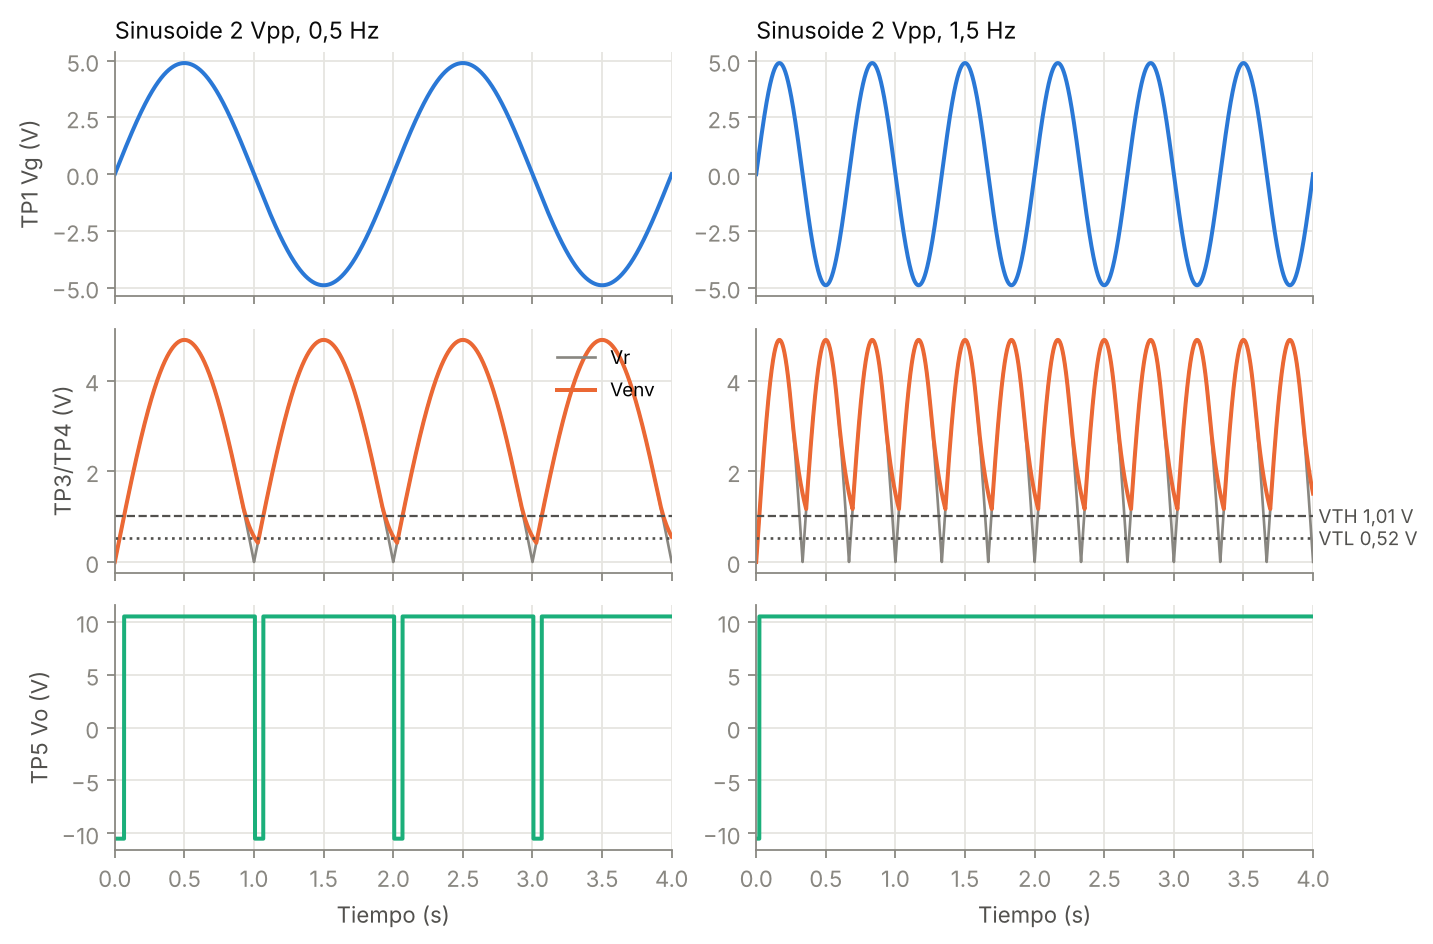
\includegraphics[width=0.95\linewidth]{f6_sinusoide.png}
\caption{Sinusoide de \SI{2}{V_{pp}} a \SI{0,5}{Hz} (dos pulsos por ciclo) y a \SI{1,5}{Hz} (salida fija en alto).}\label{fig:sin}
\end{figure}

\begin{table}[H]
\centering
\caption{Resultados con sinusoide (entre paréntesis, mínimo de $\Venv$).}\label{tab:sin}
\begin{tabular}{@{}cccc@{}}
\toprule
Frecuencia & \SI{0,5}{V_{pp}} & \SI{1}{V_{pp}} & \SI{2}{V_{pp}} \\
\midrule
\SI{0,5}{Hz} & 2 pulsos/ciclo (0,11 V) & 2 pulsos/ciclo (0,21 V) & 2 pulsos/ciclo (0,42 V) \\
\SI{1,0}{Hz} & 2 pulsos/ciclo (0,20 V) & 2 pulsos/ciclo (0,41 V) & Fijo en alto (0,82 V) \\
\SI{1,5}{Hz} & 2 pulsos/ciclo (0,29 V) & Fijo en alto (0,58 V) & Fijo en alto (1,17 V) \\
\bottomrule
\end{tabular}
\end{table}

\begin{figure}[H]
\centering
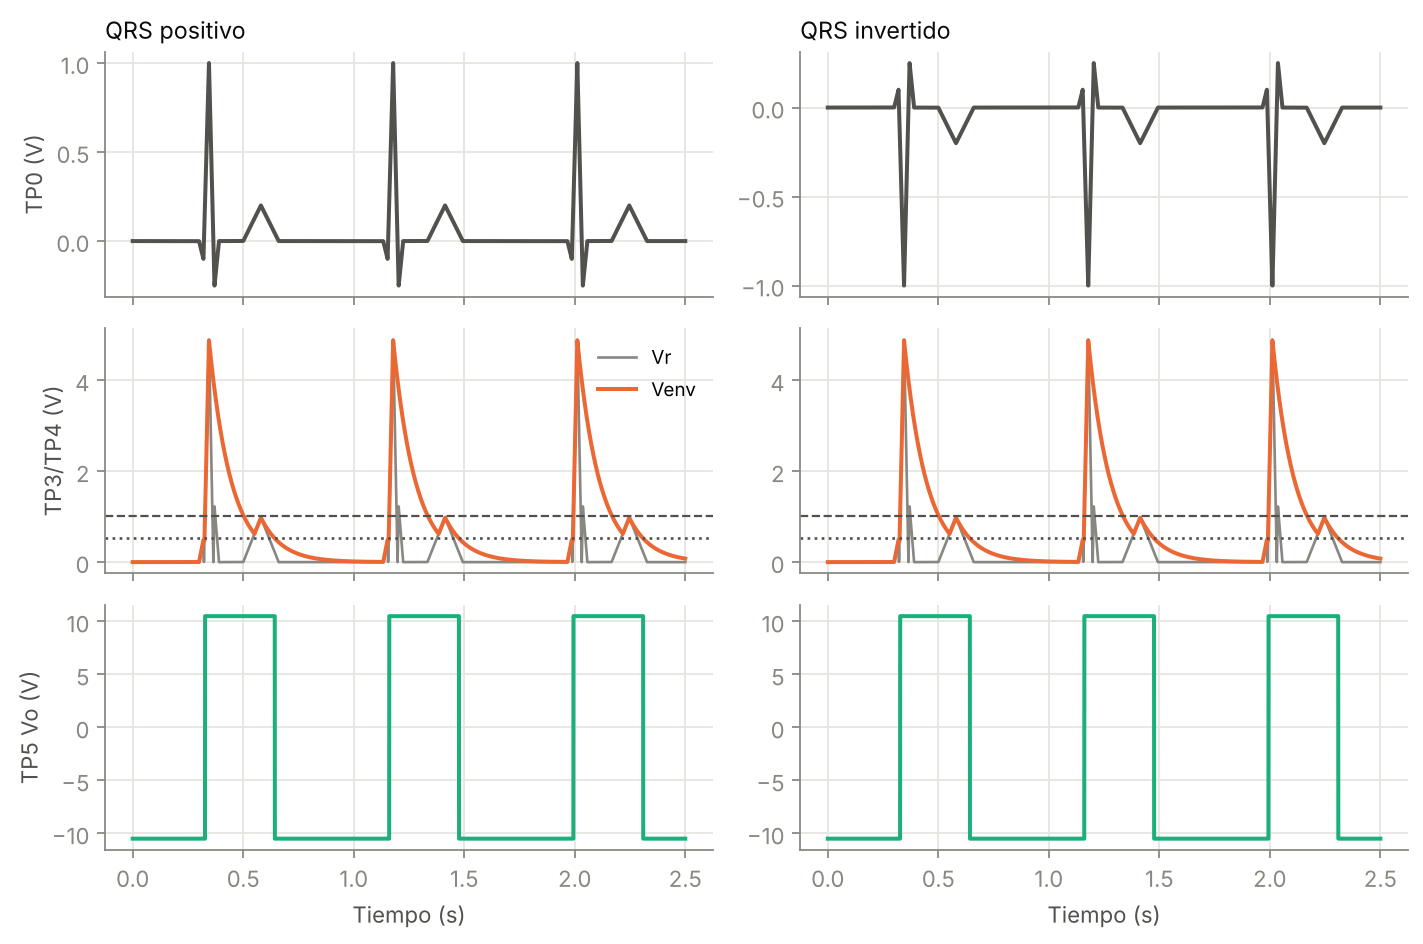
\includegraphics[width=0.95\linewidth]{f7_qrs_pwlin.png}
\caption{Latido sintético con QRS positivo e invertido: un solo pulso por latido en ambos casos.}\label{fig:qrs}
\end{figure}

Con un latido sintético (QRS de \SI{1}{V} con ondas Q y S negativas y onda T de \SI{0,2}{V}) el circuito da un pulso por latido en ambas polaridades. La onda T llega a \SI{0,98}{V} después de la ganancia, justo por debajo de $\VTH$, y cae mientras $\Venv$ sigue sobre $\VTL$, así que solo alarga el pulso.

\subsection{Simulación en Proteus}

\paragraph{Modelo de op-amp.} En Proteus se usó el modelo LM741 (un amplificador por integrado, pin 7 a $+\SI{12}{V}$ y pin 4 a $-\SI{12}{V}$). A las frecuencias de este circuito sus parámetros relevantes (slew rate de \SI{0,5}{V/\micro s}, $\Vsat\approx\pm\SI{10}{V}$, corriente de polarización de unos \SI{80}{nA}) son equivalentes a los del LM324 y el TL074 del montaje.

\paragraph{Esquema simulado.} La figura~\ref{fig:proteusesq} muestra el circuito montado en Proteus. Los nombres de los integrados los asignó el programa y no coinciden con los del informe; la equivalencia está en la tabla~\ref{tab:equiv}. El canal D del osciloscopio está conectado después de D5 (nodo del LED), por eso en las capturas el nivel bajo de la salida se lee como \SI{0}{V} en lugar de $-\Vsat$.

\begin{table}[H]
\centering
\caption{Equivalencia entre la numeración del informe y la de Proteus.}\label{tab:equiv}
\begin{tabular}{@{}lll@{}}
\toprule
Función & Informe & Proteus \\
\midrule
Amplificador & U1 & U1 \\
Media onda & U2 & U5 \\
Sumador & U3 & U4 \\
Detector & U4 & U9 \\
Buffer & U5 & U2 \\
Schmitt & U6 & U7 \\
LED & LED1 & D6 (LED-AQUA) \\
\bottomrule
\end{tabular}
\end{table}

\paragraph{Fuentes de prueba.}
\begin{itemize}
  \item \textbf{PULSE:} nivel bajo \SI{0}{V}; nivel alto 0,5, 1 o \SI{2}{V} ($-\SI{1}{V}$ para la polaridad negativa); flancos de \SI{10}{\micro s}; ancho del \SI{9}{\percent} del periodo o fijo de \SI{75}{ms}. Las capturas de resultados se tomaron a \SI{0,5}{Hz} con \SI{9}{\percent} (\SI{180}{ms}).
  \item \textbf{SINE:} offset 0, amplitud pico a pico de 0,5 a \SI{2}{V}, frecuencia \SI{0,5}{Hz} (y 1 o \SI{1,5}{Hz} para mostrar el límite de $\tau$).
  \item \textbf{FILE:} archivo de texto con 12 latidos sintéticos (tiempo y tensión), con la opción \emph{Repeat Waveform} activada.
\end{itemize}

\paragraph{Instrumentos.} Osciloscopio virtual con A en la entrada o TP1, B en TP3, C en TP4 y D en TP5, todos con acople DC; base de tiempo de \SI{200}{ms/div} (\SI{500}{ms/div} para la sinusoide) y disparo por flanco de subida en el canal A.

\paragraph{Escalado de frecuencia.} Si la simulación en tiempo real es lenta, todas las frecuencias se multiplican por $k$ y C1 se divide por $k$ (es el único componente que fija tiempos). Con $k=10$: pulso de \SI{12}{Hz}, C1 $=\SI{100}{nF}$; los tiempos medidos se multiplican por 10.

\begin{landscape}
\begin{center}
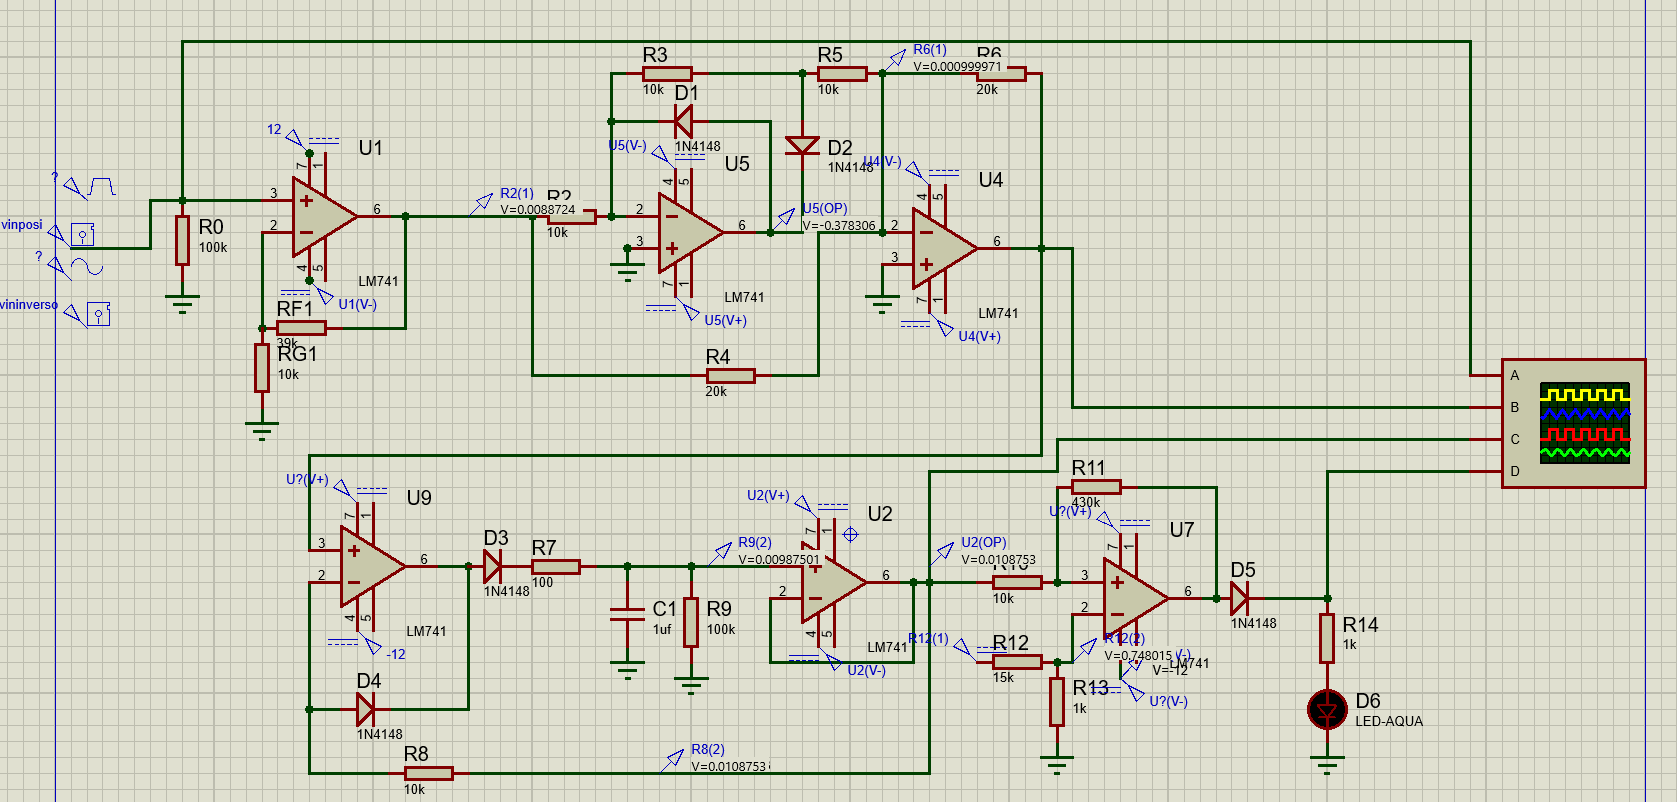
\includegraphics[width=\linewidth]{proteus_esquema.png}
\captionof{figure}{Circuito simulado en Proteus con op-amps LM741 y osciloscopio virtual (A: entrada, B: $\Vr$, C: $\Venv$, D: salida después de D5).}\label{fig:proteusesq}
\end{center}
\end{landscape}

% ---------------------------- 7. PROCEDIMIENTO -----------------------
\section{Procedimiento experimental}

\subsection{Montaje}
\begin{enumerate}
  \item Alimentar los integrados con $\pm\SI{12}{V}$ y colocar un condensador de \SI{100}{nF} entre cada pin de alimentación y tierra.
  \item Montar y verificar una etapa a la vez: comprobar TP1 antes de conectar el rectificador, y así sucesivamente.
  \item Usar tierra común entre fuente, generador y osciloscopio.
  \item Revisar la orientación de D1 a D4: un diodo invertido en el rectificador da media onda o deja la salida pegada a un riel.
  \item El circuito es solo para pruebas con generador; no se conecta a electrodos en una persona, porque eso exige aislamiento y normas de seguridad (IEC 60601).
\end{enumerate}

\subsection{Configuración del generador AFG-2025}
\begin{itemize}
  \item Pulso positivo: amplitud $=V_{pp}$ deseado, offset $=+V_{pp}/2$ (nivel bajo en \SI{0}{V}), \SI{1,2}{Hz}, ciclo de trabajo \SI{9}{\percent}.
  \item Pulso negativo: misma amplitud, offset $=-V_{pp}/2$ y ciclo de trabajo \SI{91}{\percent}.
  \item Verificar la amplitud real con el osciloscopio: si el generador está configurado para carga de \SI{50}{\ohm} y se carga con alta impedancia, entrega el doble de lo que indica.
\end{itemize}

\subsection{Puntos de medición}

\begin{table}[H]
\centering
\caption{Puntos de prueba.}\label{tab:tp}
\begin{tabularx}{\linewidth}{@{}llX@{}}
\toprule
TP & Nodo & Qué medir \\
\midrule
TP0 & Entrada & $V_{pp}$ real, frecuencia y ancho del pulso \\
TP1 & Salida de U1 ($\Vg$) & Amplitud y ganancia real \\
TP2 & Media onda ($V_{hw}$) & Solo el semiciclo positivo de $\Vg$, invertido \\
TP3 & Salida de U3 ($\Vr$) & $|\Vg|$, sin escalón en el cruce por cero \\
TP4 & Salida de U5 ($\Venv$) & Pico y $\tau$ (tiempo hasta el \SI{37}{\percent} del pico) \\
TP5 & Salida de U6 & Niveles $\pm\Vsat$, ancho de pulso y frecuencia \\
\bottomrule
\end{tabularx}
\end{table}

Con un osciloscopio de dos canales se mide en pares consecutivos (TP0--TP1, TP1--TP3, TP3--TP4, TP4--TP5) con disparo en el canal 1. Los umbrales se miden en modo XY ($X=$ TP4, $Y=$ TP5) con una rampa lenta a la entrada del Schmitt. El offset se mide en TP4 con la entrada a \SI{0}{V}.

% ---------------------------- 8. RESULTADOS --------------------------
\section{Resultados}

\subsection{Simulación en Proteus}

\paragraph{Pulso de \SI{1}{V} a \SI{0,5}{Hz}.} Con un ciclo de trabajo del \SI{9}{\percent} el pulso dura $w=0{,}09\times\SI{2}{s}=\SI{180}{ms}$. El ancho esperado de la salida es
\begin{equation}
w+\tau\ln\frac{V_p}{\VTL}=\SI{180}{ms}+\SI{100}{ms}\cdot\ln\frac{4{,}95}{0{,}523}=\SI{180}{ms}+\SI{225}{ms}=\SI{405}{ms}
\end{equation}
En la captura (figura~\ref{fig:proteuspulso}) la salida permanece en alto unos \SI{400}{ms}, $\Vr$ llega a \SI{4,90}{V} y $\Venv$ a \SI{4,95}{V}; la envolvente se mantiene plana durante el pulso y luego cae de forma exponencial.

\begin{figure}[H]
\centering
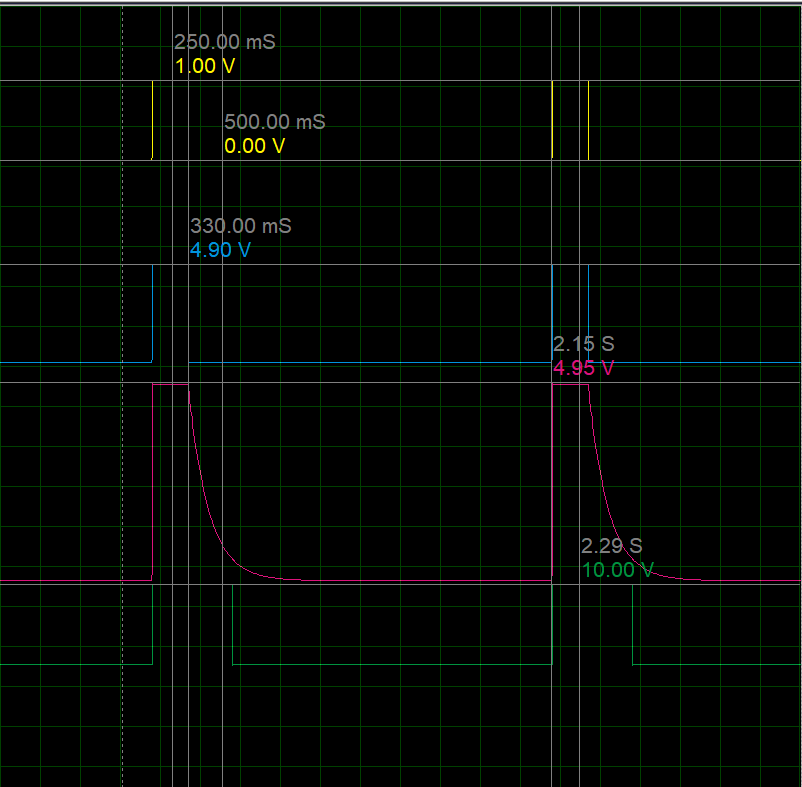
\includegraphics[width=0.78\linewidth]{proteus_pulso.png}
\caption{Proteus, pulso de \SI{1}{V} a \SI{0,5}{Hz}. Amarillo: entrada; azul: $\Vr$ (TP3); rosa: $\Venv$ (TP4); verde: salida después de D5.}\label{fig:proteuspulso}
\end{figure}

\paragraph{Sinusoide de \SI{2}{V_{pp}} a \SI{0,5}{Hz}.} $\Vr$ muestra las dos jorobas positivas por ciclo con pico de \SI{4,90}{V}, lo que confirma la rectificación de onda completa. La salida está en alto casi todo el tiempo y baja brevemente cerca de cada cruce por cero, cuando $\Venv$ cae por debajo de $\VTL$: hay dos flancos de subida por ciclo, uno por semiciclo (figura~\ref{fig:proteusseno}).

\begin{figure}[H]
\centering
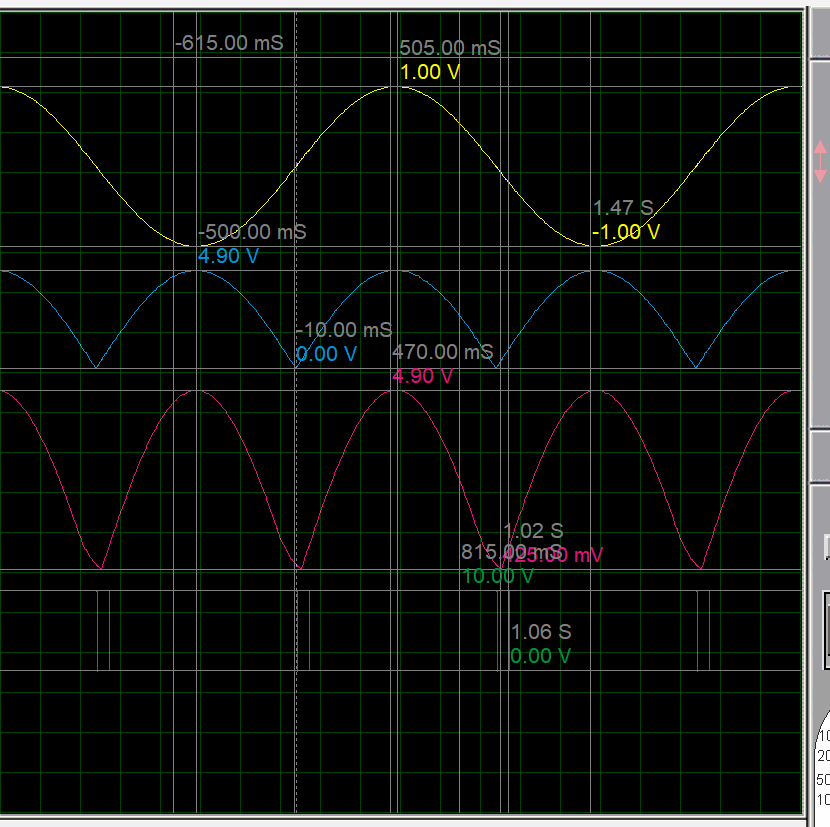
\includegraphics[width=0.78\linewidth]{proteus_seno.png}
\caption{Proteus, sinusoide de \SI{2}{V_{pp}} a \SI{0,5}{Hz}: dos pulsos de salida por ciclo.}\label{fig:proteusseno}
\end{figure}

\paragraph{Latido sintético (generador FILE).} Con el archivo de 12 latidos (QRS de \SI{1}{V}, ondas Q y S negativas y onda T de \SI{0,2}{V}), $\Vr$ muestra los lóbulos rectificados y la onda T, pero $\Venv$ los funde en una sola joroba por latido. La salida da un pulso por latido de unos \SI{325}{ms} y la onda T no produce disparos falsos (figura~\ref{fig:proteusecg}).

\begin{figure}[H]
\centering
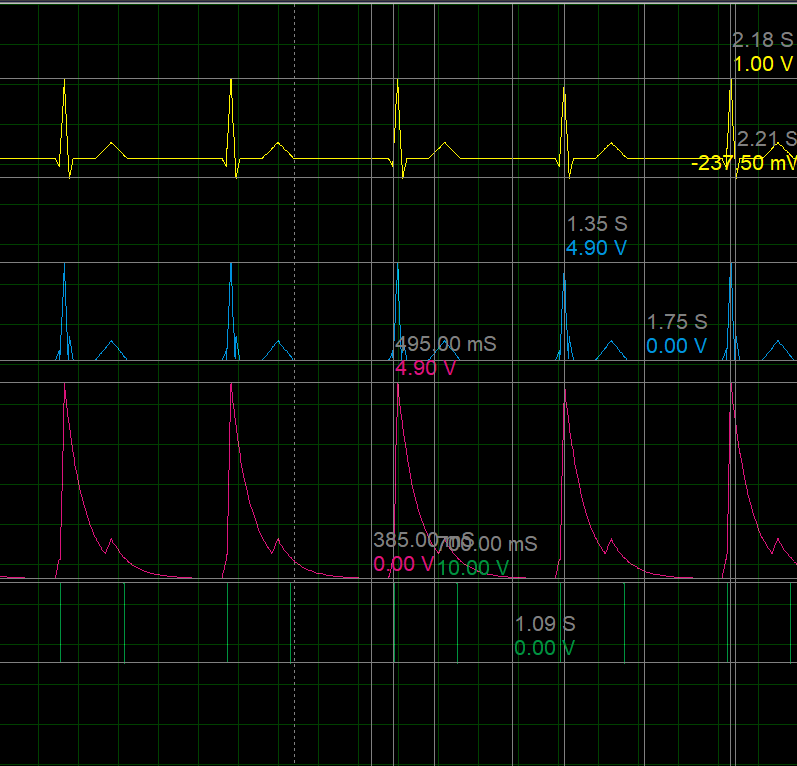
\includegraphics[width=0.78\linewidth]{proteus_ecg.png}
\caption{Proteus, latido sintético a 72 lpm: un pulso de salida por latido.}\label{fig:proteusecg}
\end{figure}

\begin{table}[H]
\centering
\caption{Comparación entre valores teóricos, simulados en Proteus y medidos en el laboratorio.}\label{tab:comparacion}
\small
\begin{tabular}{@{}lcccc@{}}
\toprule
Magnitud & Teórico & Proteus & Error (\%) & Medido \\
\midrule
\multicolumn{5}{@{}l}{\textit{Pulso de \SI{1}{V}, \SI{0,5}{Hz}, ancho \SI{180}{ms}}} \\
Ganancia $\Vr/V_{in}$ & 4,90 & 4,90 & 0,0 & \\
Pico de $\Vr$ (TP3) & \SI{4,90}{V} & \SI{4,90}{V} & 0,0 & \\
Pico de $\Venv$ (TP4) & \SI{4,90}{V} & \SI{4,95}{V} & 1,0 & \\
Ancho de pulso de salida & \SI{405}{ms} & $\approx\SI{400}{ms}$ & 1,2 & \\
Periodo de la salida & \SI{2}{s} (30 lpm) & \SI{2}{s} & 0,0 & \\
\midrule
\multicolumn{5}{@{}l}{\textit{Sinusoide de \SI{2}{V_{pp}}, \SI{0,5}{Hz}}} \\
Pico de $\Vr$ & \SI{4,90}{V} & \SI{4,90}{V} & 0,0 & \\
Pulsos por ciclo & 2 & 2 & --- & \\
\midrule
\multicolumn{5}{@{}l}{\textit{Latido sintético, 72 lpm}} \\
Pulsos por latido & 1 & 1 & --- & \\
Ancho de pulso de salida & $\approx\SI{320}{ms}$ & $\approx\SI{325}{ms}$ & 1,6 & \\
\midrule
\multicolumn{5}{@{}l}{\textit{Medidas adicionales en el laboratorio}} \\
$\tau$ de descarga & \SI{100}{ms} & & & \\
$\VTH$ & \SI{1,01}{V} & & & \\
$\VTL$ & \SI{0,52}{V} & & & \\
Offset en TP4 (entrada a \SI{0}{V}) & $<\SI{50}{mV}$ & & & \\
\bottomrule
\end{tabular}
\end{table}

\subsection{Montaje en el laboratorio}

\begin{figure}[H]
\centering
\pendiente{Insertar fotografía del montaje en la protoboard.}
\caption{Montaje del detector en la protoboard.}\label{fig:montaje}
\end{figure}

\begin{figure}[H]
\centering
\pendiente{Insertar captura del osciloscopio del laboratorio: pulso a la entrada y salida del detector.}
\caption{Medición en el montaje: respuesta al pulso.}\label{fig:medpulso}
\end{figure}

\begin{figure}[H]
\centering
\pendiente{Insertar captura del osciloscopio del laboratorio: sinusoide a la entrada y salida del detector.}
\caption{Medición en el montaje: respuesta a la sinusoide.}\label{fig:medseno}
\end{figure}

% ---------------------------- 9. ANALISIS ----------------------------
\section{Análisis y discusión}

\subsection{Límites de frecuencia}
El límite superior lo fija la condición $w+t_{desc}<T$ (ecuación~\ref{eq:fcmax}): con el pulso de ancho fijo de \SI{75}{ms} es de 262, 201 y 163 lpm para 0,5, 1 y \SI{2}{V_{pp}}. Baja con la amplitud porque un pico mayor tarda más en descargarse: duplicar el pico añade $\tau\ln2\approx\SI{69}{ms}$. No hay límite inferior real, porque el circuito está acoplado en DC; solo se requiere que el pulso dure al menos $\approx\SI{0,5}{ms}$ para cargar C1. La sinusoide tiene un límite más bajo que el pulso porque produce dos eventos por ciclo y la señal casi nunca está en cero.

\subsection{Comparación de op-amps}\label{sec:opamps}

\begin{table}[H]
\centering
\caption{Op-amps considerados.}\label{tab:opamps}
\begin{tabularx}{\linewidth}{@{}lllX@{}}
\toprule
Parámetro & TL074 & LM324 / LM741 & Efecto en el circuito \\
\midrule
Corriente de polarización & $\approx\SI{30}{pA}$ & 45--\SI{80}{nA} & Error en C1 menor que \SI{0,2}{\percent} en ambos \\
Slew rate & \SI{13}{V/\micro s} & \SI{0,5}{V/\micro s} & Transiciones de \si{\micro s}: despreciables \\
Salida a $\pm\SI{12}{V}$ & $\pm\SI{10,5}{V}$ & $\approx\pm10$ a \SI{11,5}{V} & Mueve los umbrales unos mV \\
Offset en $\Venv$ & 15--\SI{20}{mV} & 20--\SI{45}{mV} típico & Muy por debajo de $\VTL$ \\
\bottomrule
\end{tabularx}
\end{table}

\subsection{Limitaciones}
\begin{itemize}
  \item Umbrales fijos: por debajo de $\approx\SI{0,4}{V_{pp}}$ no hay detección y por encima de $\approx\SI{2,1}{V_{pp}}$ U1 se satura. Un monitor real usa un umbral adaptativo (una fracción del pico anterior).
  \item $\tau$ fijo limita la frecuencia máxima a $\approx163$ lpm con \SI{2}{V_{pp}}.
  \item Sin filtrado: con una señal real, una onda T alta o el ruido de \SI{60}{Hz} podrían disparar el comparador. Un monitor real antepone un amplificador de instrumentación y un filtro pasa banda de 0,5 a \SI{40}{Hz}.
  \item Con el 741, el peor caso de corriente de polarización por R0 puede llevar el offset a $\approx\SI{0,27}{V}$; si es un problema, R0 puede bajarse a \SI{10}{k\ohm} sin afectar el resto.
\end{itemize}

% ---------------------------- 10. CONCLUSIONES -----------------------
\section{Conclusiones}
\begin{itemize}
  \item Se diseñó un detector de latido que entrega un pulso por cada complejo QRS usando solo bloques no lineales con op-amps. En Proteus los valores coincidieron con los calculados con errores de 1,6\,\% o menos: picos de \SI{4,90}{V} en $\Vr$ y \SI{4,95}{V} en $\Venv$, y un pulso de salida de unos \SI{400}{ms} frente a los \SI{405}{ms} predichos.
  \item El rectificador de precisión de onda completa resolvió el problema de la polaridad: la sinusoide dio dos pulsos por ciclo y el latido sintético invertido se detectó igual que el positivo. Colocar el diodo dentro del lazo de realimentación reduce la zona muerta de \SI{0,6}{V} a unos \si{\micro V}; un rectificador pasivo habría perdido el \SI{25}{\percent} de la señal más pequeña.
  \item El sumador muestra cómo una operación lineal produce una función no lineal: combinar la señal completa (peso 1) con la media onda (peso 2) da $|\Vg|$. El análisis también mostró que el semiciclo positivo depende de una resta ($2-1$), por lo que las resistencias deben ser al \SI{1}{\percent}.
  \item La constante de descarga $\tau=R_9C_1$ es el parámetro crítico. No se eligió arbitrariamente: la ventana de 90 a \SI{110}{ms} sale de dos condiciones opuestas, fundir los lóbulos del QRS y liberar el comparador antes del siguiente latido. La fórmula $FC_{max}=60/(w+\tau\ln(V_p/\VTL))$ predijo correctamente el único caso de falla de la simulación (180 lpm con \SI{2}{V_{pp}}).
  \item El buffer y la resistencia R8 son indispensables: el buffer impide que R8 y el comparador descarguen el condensador (sin él $\tau$ caería a unos \SI{9}{ms}), y R8 permite que la salida del buffer y la tierra virtual del detector tengan tensiones distintas durante la descarga.
  \item La realimentación positiva del comparador Schmitt da dos umbrales (\SI{1,01}{V} y \SI{0,52}{V}) y transiciones regenerativas: al disparar, la entrada no inversora salta lejos de la referencia y el ruido no puede devolver la salida. Con la onda T del latido sintético no hubo disparos falsos.
  \item El diseño tiene límites claros: umbrales fijos (entradas de 0,4 a \SI{2,1}{V_{pp}}), frecuencia máxima de unos 160 lpm con la amplitud mayor y ausencia de filtrado. Un siguiente paso sería anteponer un amplificador de instrumentación con filtro pasa banda de 0,5 a \SI{40}{Hz}, usar un umbral adaptativo y contar los pulsos con un microcontrolador para mostrar la frecuencia cardiaca.
\end{itemize}

% ---------------------------- REFERENCIAS ----------------------------
\begin{thebibliography}{10}
\bibitem{sedra} A. S. Sedra y K. C. Smith, \emph{Microelectronic Circuits}, Oxford University Press.
\bibitem{franco} S. Franco, \emph{Design with Operational Amplifiers and Analog Integrated Circuits}, McGraw-Hill.
\bibitem{boylestad} R. L. Boylestad y L. Nashelsky, \emph{Electrónica: teoría de circuitos y dispositivos electrónicos}, Pearson.
\bibitem{guyton} J. E. Hall y M. E. Hall, \emph{Guyton y Hall. Tratado de fisiología médica}, Elsevier. Capítulo: el electrocardiograma normal.
\bibitem{pantompkins} J. Pan y W. J. Tompkins, ``A Real-Time QRS Detection Algorithm'', \emph{IEEE Transactions on Biomedical Engineering}, vol. BME-32, n.\textsuperscript{o} 3, pp. 230--236, 1985.
\bibitem{webster} J. G. Webster (ed.), \emph{Medical Instrumentation: Application and Design}, Wiley.
\bibitem{tl074} Texas Instruments, \emph{TL07xx Low-Noise FET-Input Operational Amplifiers}, hoja de datos.
\bibitem{lm324} Texas Instruments, \emph{LMx24 Quadruple Operational Amplifiers}, hoja de datos.
\bibitem{lm741} Texas Instruments, \emph{LM741 Operational Amplifier}, hoja de datos.
\bibitem{1n4148} Vishay / onsemi, \emph{1N4148 Small Signal Fast Switching Diode}, hoja de datos.
\end{thebibliography}

% ---------------------------- ANEXOS --------------------------------
\appendix
\newpage
\section{Código de la simulación por comportamiento}\label{anx:codigo}
El siguiente script genera las figuras y tablas de la sección de simulación.
\lstinputlisting[language=Python]{../simulacion/sim.py}

\section{Archivos de latido sintético para Proteus}
Los archivos \texttt{ecg\_latido\_positivo.txt} y \texttt{ecg\_latido\_invertido.txt} contienen 12 latidos a 72 lpm (\SI{10}{s}). Cada línea tiene el tiempo en segundos y la tensión en voltios. Puntos de un latido:

\begin{table}[H]
\centering
\caption{Puntos de un latido sintético.}\label{tab:pwlin}
\begin{tabular}{@{}cccccccccc@{}}
\toprule
$t$ (s) & 0 & 0,300 & 0,320 & 0,345 & 0,370 & 0,390 & 0,500 & 0,580 & 0,660 \\
$V$ (V) & 0 & 0 & $-0{,}10$ & 1,00 & $-0{,}25$ & 0 & 0 & 0,20 & 0 \\
\bottomrule
\end{tabular}
\end{table}

\end{document}
